\chapter{Instrument Sensitivity}
\label{ch:cmb_instrument_sensitivity}

As overviewed in Section~\ref{sec:simons_array}, telescopes for observation of CMB polarization anisotropies are complex systems that rely on high-quality optical, thermal, and detection performance to be successful. Instrument performance is typically broken into two categories: \important{sensitivity} and \important{systematics}. Sensitivity is a simplistic measure of the instrument's signal to noise and relies, at its core, on only two factors: the amount of noise in your detectors, and the optical throughput of the system to a given signal on the sky. Sensitivity analyses typically assume a white noise spectrum (in other words, that all noise fluctuations are Gaussian, uncorrelated, and equal across all time scales) and a fixed sky signal. Systematics, on the other hand, are substantially more complex and involve effects such as optical sidelobes, intensity-to-polarization leakage, cross polarization, scan-synchronous signal, low-frequency noise, detector gain drift, focal plane temperature changes, readout pathologies, etc. In this sense, an accurate analyses of systematic effects requires a deep knowledge of the instrument and is a prerequisite to understanding not only system performance but the science data itself.

As detailed in Chapter~blah, a primary product of this dissertation is the development of a sensitivity calculator useful for both instrument design and forecasting and for instrument characterization. As a precursor to that discussion, we present the sensitivity calculation itself in this chapter, noting key advancements made as part of the presented research.

%%%%%%%%%%%%%%%%%%%%%%%%%%%%%%%%
%%%%%%%%%%%%%%%%%%%%%%%%%%%%%%%%
%%%%%%%%%%%%%%%%%%%%%%%%%%%%%%%%

\section{Noise spectrm}
\label{sec:sensitivity_noise_spectrum}

Sensitivity is often quantified in terms of the instrument's signal-to-noise ratio (SNR). In experiments that use photodetectors, such as mm-wave telescopes, SNR is often expressed in terms of \important{noise-equivalent power}, which is defined to be the signal power that gives a SNR of one given one Hz of output bandwidth. In this sense, NET is spectral quantity, and the amount of noise in a given sample depends on both the shape of the noise spectrum and on the integration bandwidth
\begin{equation}
    \left< \sigma_{\mathrm{P}}^{2} \right> = \int_{f_{\mathrm{lo}}}^{f_{\mathrm{hi}}} \left| \mathrm{NEP}(f) \right|^{2} \dd f \, ,
    \label{eq:net_spectrum_integrate}
\end{equation}
where here $f$ is \important{audio frequency} (in contrast to \textit{microwave frequencies}, which describe the vibrations of electromagnetic radiation).

When estimate the sensitivity of CMB instruments, the noise is often approximated to be ``white,'' or independent of frequency. In this case, the integral in Equation~\ref{eq:net_spectrum_integrate} becomes
\begin{equation}
    \left< \sigma_{\mathrm{P}}^{2} \right> = \left| \mathrm{NEP}\right|^{2} \Delta f \, ,
    \label{eq:net_white_spectrum}
\end{equation}
where $\Delta f$ is the \important{output bandwidth}. To understand the meaning of the output bandwidth, consider the Nyquist sampling theorem, which relates the \textit{maximum} integration bandwidth $\Delta f_{\mathrm{max}}$ to the sampling rate $1 / \Delta t_{\mathrm{samp}}$ as
\begin{equation}
    \Delta f_{\mathrm{max}} = \frac{1}{2 \Delta t_{\mathrm{samp}}} \, ,
    \label{eq:output_bandwidth_nyquist_frequency}
\end{equation}
When $\Delta f = f_{2} - f_{1} = f_{\max} - 0$, as is often the case when measuring an unmodulated signal, $f_{\mathrm{max}}$ is called the \important{Nyquist Frequency}.

NEP in CMB experiments is generally decomposed into photon noise, bolometer thermal noise, readout/amplifier noise, TES Johnson noise, and extraneous noise sources, each of which we detail in the sections to follow. These noise sources are typically assumed to be white and uncorrelated, meaning that they can be simulated independently and that their amplitudes add in quadrature. After estimating the NEP of a given detector output, it is then useful to estimate instrument signal to noise in terms of a given sky signal, which which is often given in temperature units and is referred to as \important{noise-equivalent temperature} (NET). NET is a common figure of merit for instrument sensitivity, and an accurate estimate relies on an accurate understanding of many aspects of the instrument, including the ambient optical environment, telescope + receiver optical throughput, bolometer and SQUID noise, spillover both inside and outside of the cryostat, and beam coupling efficiency (see Equation~\ref{eq:beam_coupling_efficiency}).

%%%%%%%%%%%%%%%%%%%%%%%%%%%%%%%%
%%%%%%%%%%%%%%%%%%%%%%%%%%%%%%%%
%%%%%%%%%%%%%%%%%%%%%%%%%%%%%%%%

\section{Photon statistics}
\label{sec:sensitivity_photon_statistics}

As briefly alluded to in Section~\ref{sec:sensitivity_optical_power_detail}, it is often convenient to describe the propagation of radiation through the optical system to the detector in terms of \important{modes}. A single mode of the electric field is given by
\begin{equation}
    E_{p}(\vec{r}, t) = E_{0} \sin \left( \vec{k} \cdot \vec{r} - \omega t \right) \, ,
    \label{eq:electromagnetic_mode}
\end{equation}
where $\vec{r}$ is position, $t$ is time, $\vec{k} = (2 \pi \nu / c) \hat{k}$ is the wave vector, $\omega = c k$ is the light's angular frequency, and the index $p$ denotes a single polarization. The important characteristic of an electromagnetic mode is that it is described by a single vibrational component of microwave frequency $\nu$ and is therefore best represented in frequency space.

The quantum mechanical analog to electromagnetic modes are \important{coherent states}, which, as the name suggests, is a basis of full coherence. Coherent states are eigenvectors of the photon creation operator $a^{\dagger}_{\vec{k} p}$
\begin{equation}
    a^{\dagger}_{\vec{k} p} \left| \alpha_{\vec{k} p} \right> = \alpha_{\vec{k} p} \left| \alpha_{\vec{k} p} \right> \, .
    \label{eq:coherent_state_eigenbasis}
\end{equation}
It is also useful to define the electric field operator as
\begin{equation}
    \hat{E}_{p}^{(+)}(\vec{r}, t) \left| \alpha_{\vec{k} p} \right> = E_{p}(\vec{r}, t) \left| \alpha_{\vec{k} p} \right> \, ,
    \label{eq:electric_field_operator_definition}
\end{equation}
where here, the classical quantity $E_{p}(\vec{r}, t)$ is the observable quantity. Given Equations~\ref{eq:coherent_state_eigenbasis} and~\ref{eq:electric_field_operator_definition}, we can relate the electric field operator for a single electromagnetic mode to the photon operator for a coherent state as
\begin{equation}
    \hat{E}_{p}^{(+)}(\vec{r}, t) = \sqrt{\frac{\hbar \omega}{2 \varepsilon_{0} v}} a_{\vec{k} p}^{\dagger} \sin(\vec{k} \cdot \vec{r} - \omega t) \, ,
    \label{eq:electric_field_operator_single_mode}
\end{equation}
where here $\hbar$ is the reduce Planck constant, $\varepsilon_{0}$ is the permittivity of free space, $v$ is the volume of space of interest. Equation~\ref{eq:electric_field_operator_single_mode} show that by understanding the quantum fluctuations of the \textit{quantum} coherent state $\left| \alpha_{\vec{k} p} \right>$, we can understand the photon noise in a \textit{classical} field $E_{p}(\vec{r}, t)$.

In order to study the statistics of thermal light, we can assume that the probability of finding a photon is governed by the Boltzmann probability distribution
\begin{equation}
    P_{n} = \frac{\exp \left( - E_{n} / k_{\mathrm{B}} T \right)}{\sum_{n = 0}^{\infty} \exp \left( - E_{n} \ k_{\mathrm{B}} T \right)} \, ,
    \label{eq:boltzmann_distribution}
\end{equation}
where the energy of the harmonic oscillator state $n$ is given by
\begin{equation}
    E_{n} = \left( n + \frac{1}{2} \right) \hbar \omega \, ,
    \label{eq:harmonic_oscillator_energy}
\end{equation}
and where here, again is related to microwave frequency as $\omega = 2 \pi \nu$. Noting that the zero-point energy cancels out when Equation~\ref{eq:harmonic_oscillator_energy} is substituted into Equation~\ref{eq:boltzmann_distribution}, it is convenient to define the factor 
\begin{equation}
    U = \exp \left(- \hbar \omega / k_{\mathrm{B}} T \right) \, ,
    \label{eq:boltzmann_energy_factor}
\end{equation}
such that the probability distribution can be rewritten as 
\begin{equation}
    P_{n} = \frac{U^{n}}{\sum_{n = 0}^{\infty} U^{n}} = \left( 1 - U \right) U^{n} \, ,
    \label{eq:boltzmann_probability_simplified}
\end{equation}
where we have invoked the geometry series relation $\sum_{n = 0}^{\infty} U^{n} = (1 - U)^{-1}$. Given this simplified form for the probability distribution, we can calculate the mean photon occupation number as
\begin{equation}
    \left< n \right> = \sum_{n = 0}^{\infty} n P_{n} = \left( 1 - U \right) \sum_{n = 0}^{\infty} n U^{n} = \frac{U}{1 - U} \, ,
    \label{eq:mean_photon_count_probability_distribution}
\end{equation}
where we have used the relation $\sum_{n} n U^{n} = U \partial / \partial U \sum_{n} U^{n}$ and have once again invoked the geometry series relation $\sum_{n = 0}^{\infty} U^{n} = (1 - U)^{-1}$. Substituting Equation~\ref{eq:boltzmann_energy_factor} into Equation~\ref{eq:mean_photon_count_probability_distribution} gives the mean photon number for thermal light of temperature $T$ at frequency $\omega$
\begin{equation}
    \left< n \right> = \frac{1}{\exp \left( \hbar \omega / k_{\mathrm{B}} T \right) - 1} \, ,
    \label{eq:photon_occupation_number}
\end{equation}
which is the familiar \important{Bose-Einsten distribution}.

\begin{figure}[!t]
    \centering
    \subfloat[\label{fig:photon_statistics:a}]{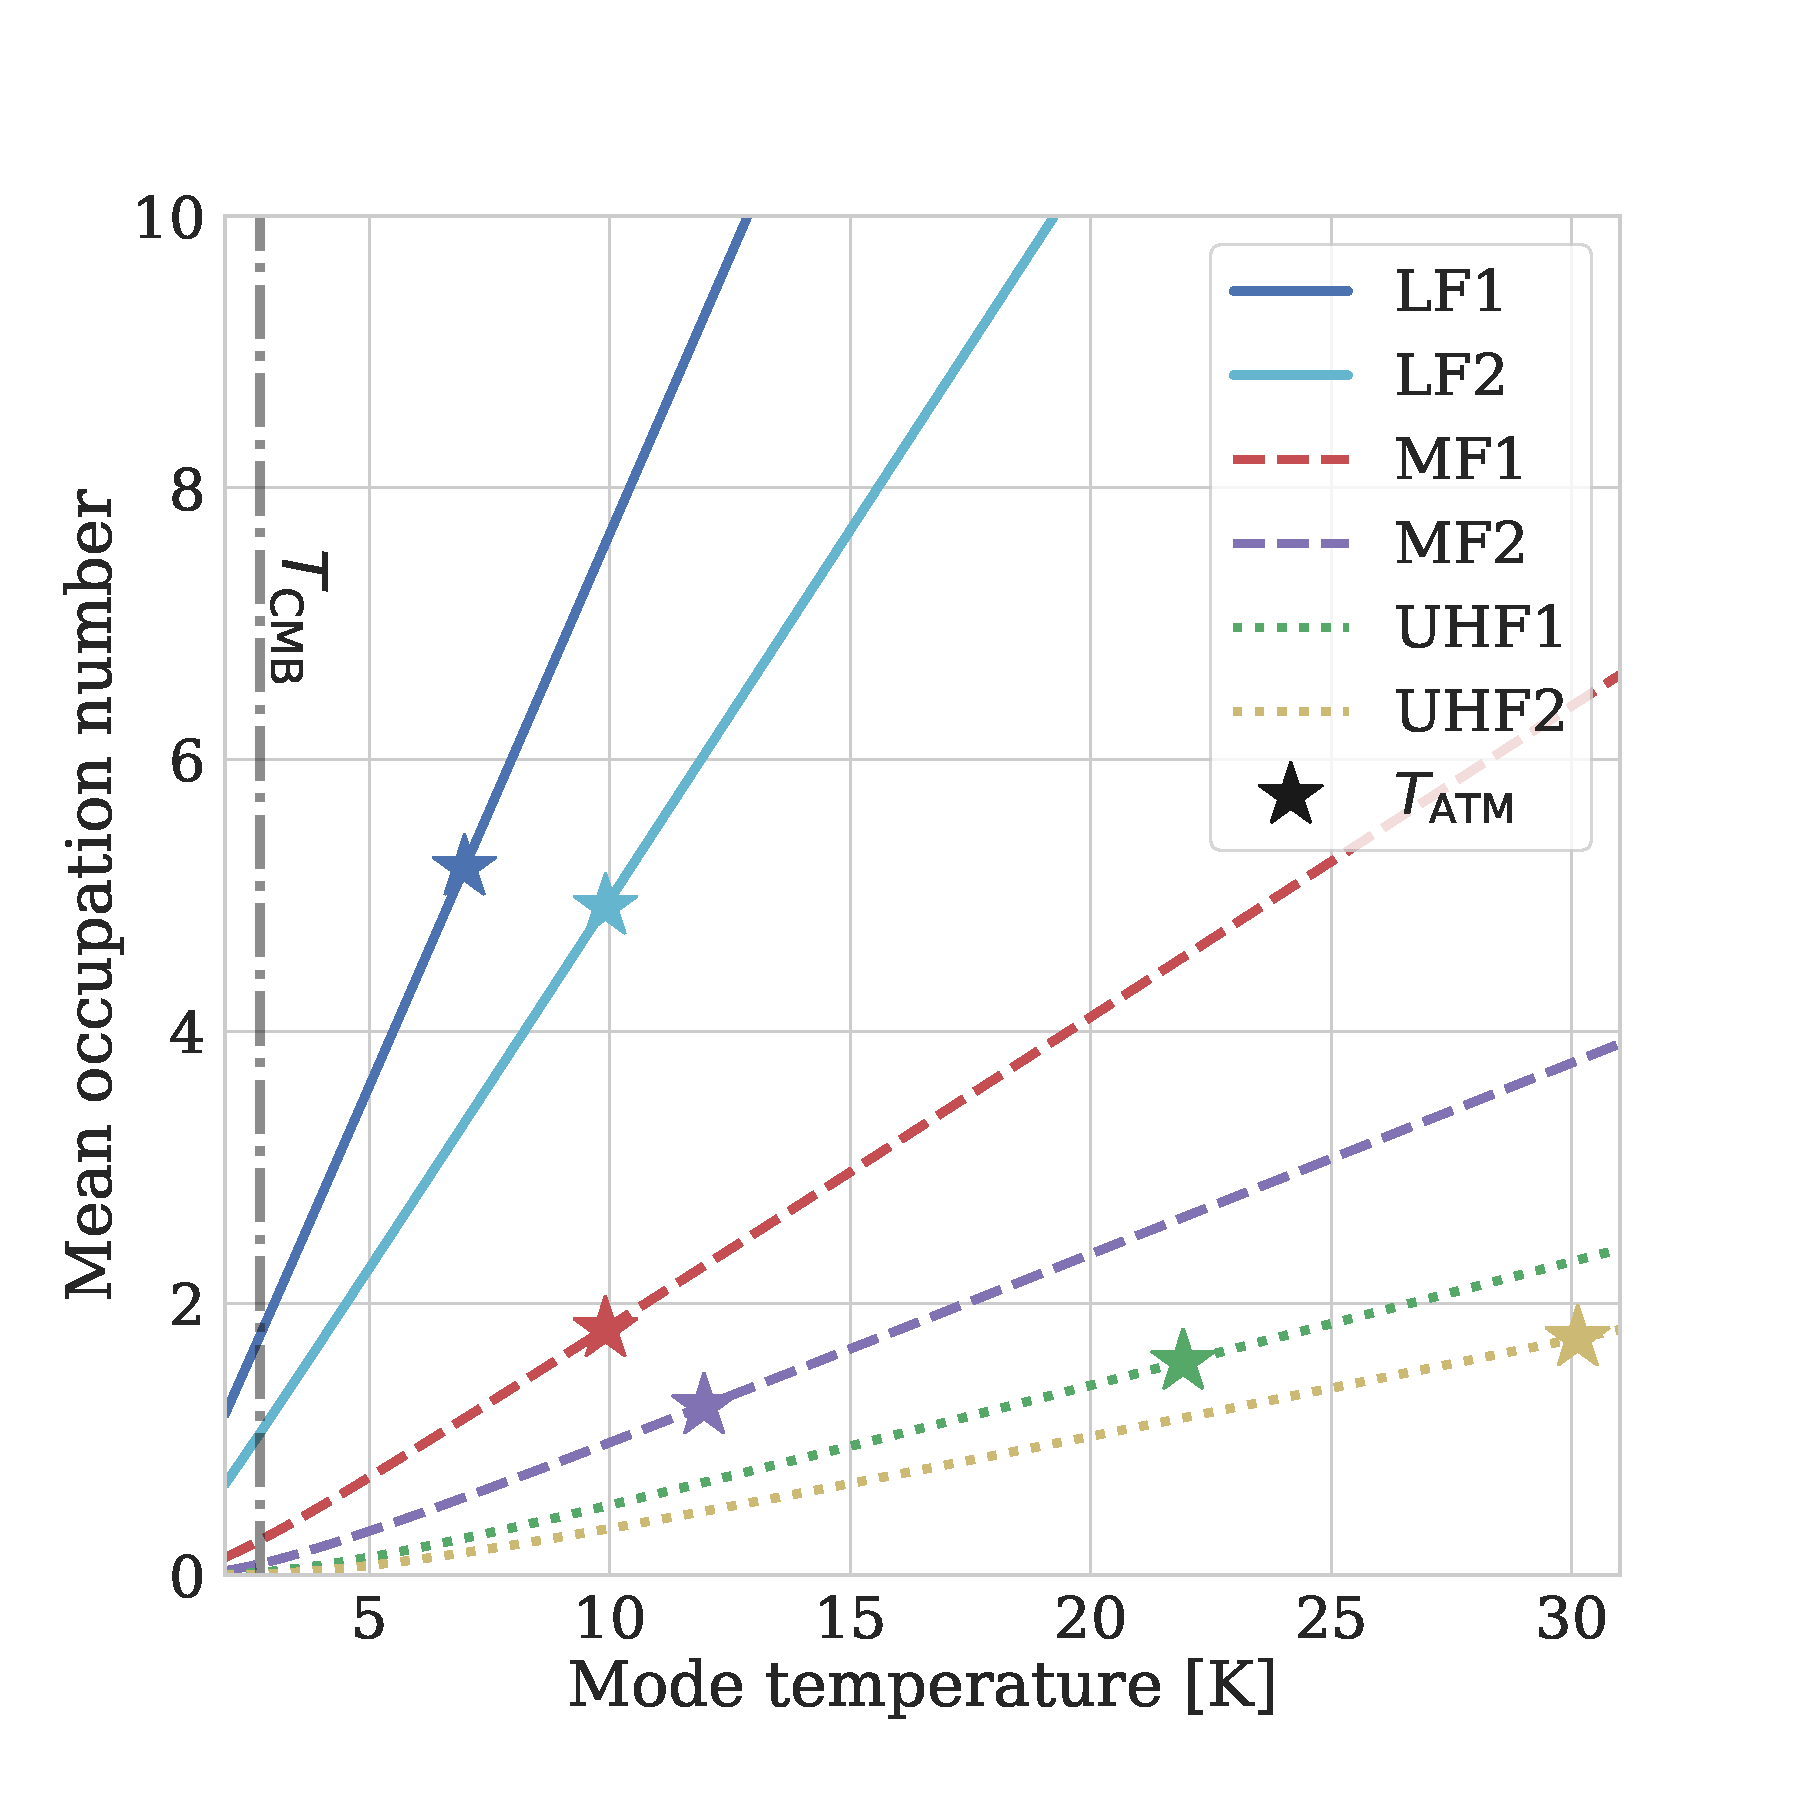
\includegraphics[width=0.48\linewidth, trim=0cm 1cm 2cm 3cm, clip]{SensitivityCalculation/Figures/mean_occupation_number.pdf}}
    \subfloat[\label{fig:photon_statistics:b}]{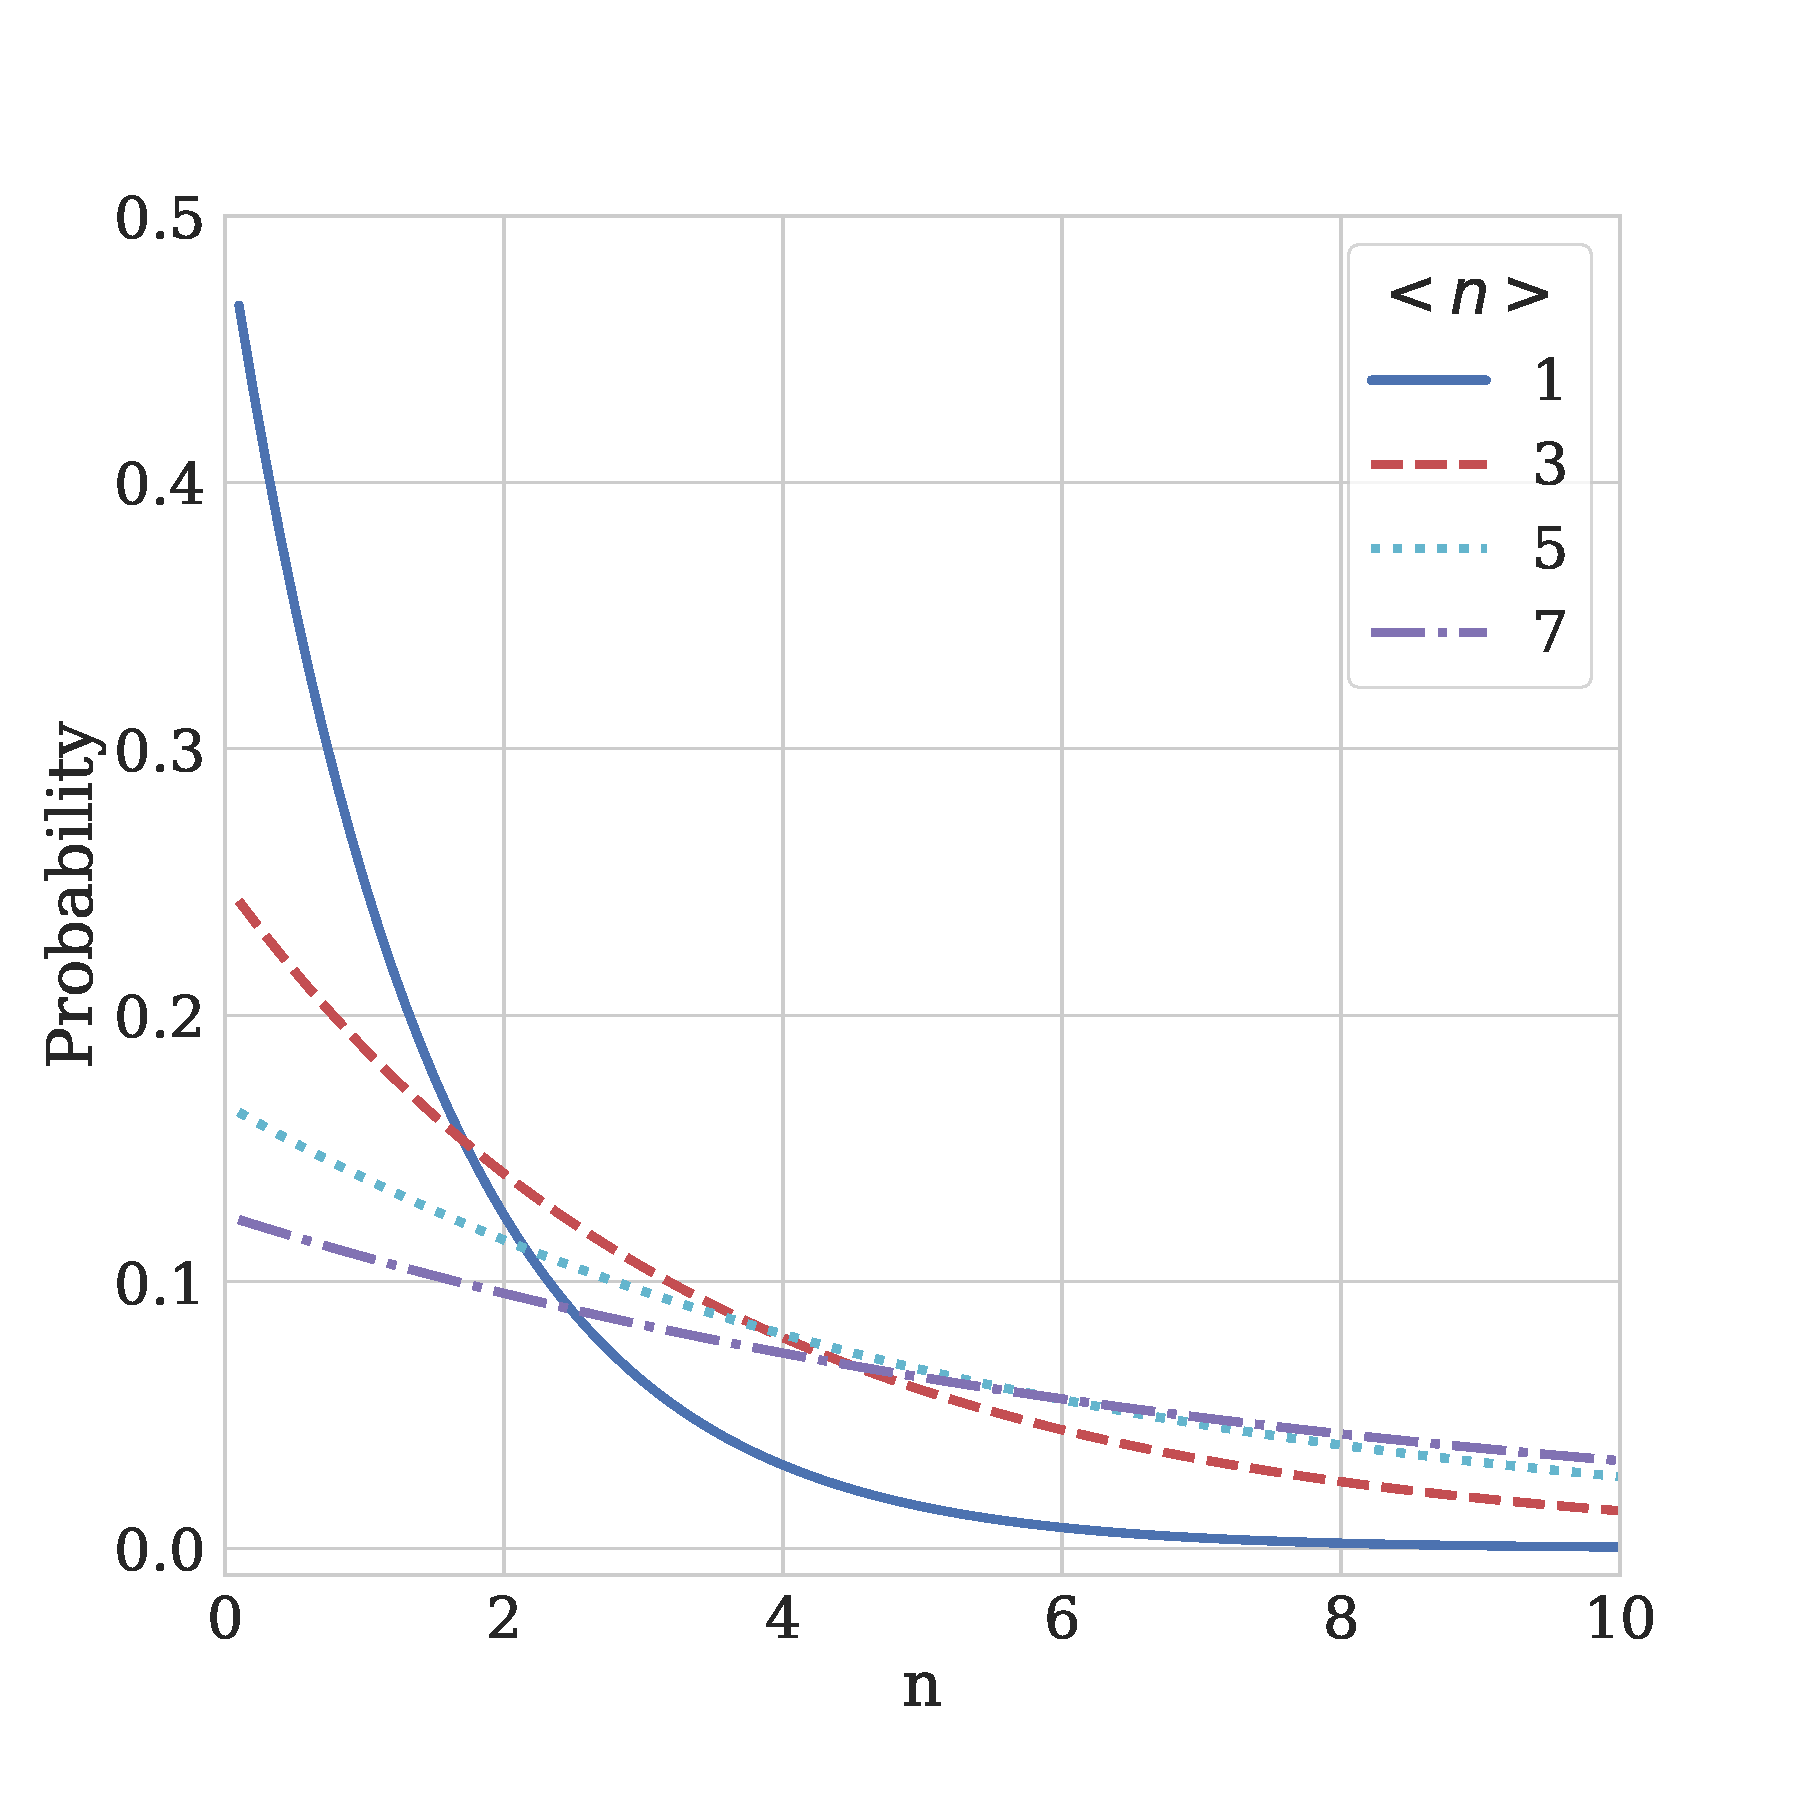
\includegraphics[width=0.48\linewidth, trim=0cm 1cm 2cm 3cm, clip]{SensitivityCalculation/Figures/occupation_number_distribution.pdf}}
    \caption{(a) is the mean occupation number vs mode temperature integrated over the SO bands. The atmospheric temperature for each band is marked with a star, and the CMB temperature is marked with a vertical line. (b) is the probability distribution vs mode number for various mean occupation numbers. The probability broadens with increasing $\left< n \right>$, which in turn gives rise to larger mode fluctuations, while at smaller $\left< n \right>$ the distribution looks increasingly Poissonian.}
    \label{fig:my_label}
\end{figure}

Now that we have an expression for the \textit{mean} photon count, we move to find an expression for the RMS photon count fluctuations
\begin{equation}
    \left( \Delta n \right)^{2} = \sum_{n} \left(n - \left< n \right> \right)^{2} P_{n} = \left< n ^{2} \right> - \left< n \right>^{2} \, .
    \label{eq:photon_variance_probability_distribution}
\end{equation}
In order to simplify this expression, it is useful to rewrite $P_{n}$ by plugging $U = \left< n \right> \ (1 + \left< n \right>)$ into Equation~\ref{eq:boltzmann_probability_simplified} to obtain
\begin{equation}
    P_{n} = \frac{\left< n \right>^{n}}{\left( 1 + \left< n \right> \right)^{1 + n}} \, .
    \label{eq:boltzmann_probability_in_terms_of_mean}
\end{equation}
In addition, it is useful to write the $P_{n}$ in terms of its \textit{factorial moments}
\begin{equation}
    \left< \frac{n !}{\left( n - r \right) !} \right> = \sum_{n} n \left( n - 1 \right) \left( n - 2 \right) ... \left( n - r + 1 \right) P_{n} = r ! \left< n \right>^{r} \, ,
    \label{eq:factorial_moments_boltzmann}
\end{equation}
where the last equality comes from plugging Equation~\ref{eq:boltzmann_probability_in_terms_of_mean} in for $P_{n}$ (citation needed for Loudon). We can then use Equation~\ref{eq:factorial_moments_boltzmann} with $r = 2$ to find
\begin{equation}
    \left< n (n - 1) \right> = 2 \left< n \right>^{2} \, ,
    \label{eq:factorial_second_moment}
\end{equation}
which can finally be plugged into Equation~\ref{eq:photon_variance_probability_distribution} to obtain the relation
\begin{equation}
    \left( \Delta n \right)^{2} = \left< n \right> + \left< n \right>^{2} \, .
    \label{eq:photon_count_fluctuations}
\end{equation}
When the mean photon occupation number is $\left< n \right> \ll 1$, which is true when $\hbar \omega \gg k_{\mathrm{B}} T$, Equation~\ref{eq:photon_count_fluctuations} reduces to $\left( \Delta n \right)^{2} \approx \left< n \right>$, which is true of a Poisson distribution. Therefore, in the high-frequency and/or low-temperature limit, photon noise is \important{shot noise} and fluctuations are uncorrelated. On the other hand, when the occupation is $\left< n \right> \gg 1$, which is true when $\hbar \omega \ll k_{\mathrm{B}} T$, Equation~\ref{eq:photon_count_fluctuations} reduces to $\left( \Delta n \right)^{2} \approx \left< n \right>^{2}$, which is true of an exponential distribution. Therefore, in the low-frequency and/or high-temperature limit, photon noise is (what is often called) \important{Bose noise} and fluctuations are, in general, correlated.

%%%%%%%%%%%%%%%%%%%%%%%%%%%%%%%%
%%%%%%%%%%%%%%%%%%%%%%%%%%%%%%%%
%%%%%%%%%%%%%%%%%%%%%%%%%%%%%%%%

\section{Photon NEP}
\label{sec:sensitivity_photon_nep}

According to Equation~\ref{eq:photon_count_fluctuations}, the variance of the photon occupation number for a given mode is determined solely by the mean occupation number. In this section, we relate those photon count statistics to those of optical power and outline the calculation of photon NEP.

Under the assumption that each optic is an isothermal blackbody, the power spectral density $p_{i}(\nu)$ for optical element $i$ is determined by its physical temperature $T_{i}$, the aggregate transmissivity of all optics between it and the detector $\left[ \eta_{i+1} (\nu) , \ldots , \eta_{N_{\mathrm{elem}}} (\nu) \right]$, its emissivity $\epsilon_{i} (\nu)$, its spillover fraction $\beta_{i} (\nu)$, the effective temperature of the spillover radiation $T_{\beta ; i}$, its scattering fraction $\delta_{i} (\nu)$, and the effective temperature of the scattered radiation $T_{\delta ; i}$
\begin{align}
    p_{i} \left( \nu \right) =
    \prod_{j = i + 1}^{N_{\mathrm{elem}}} \eta_{j} (\nu) \left[ \epsilon_{i} (\nu) S(T_{i}, \nu) + \beta_{i}(\nu) S(T_{\beta;i}, \nu) + \delta_{i}(\nu) S(T_{\delta; i}, \nu) \right] \, .
    \label{eq:pow_spec_density}
\end{align}
Here, the power spectral density function $S(T, \nu)$ of the emitted, scattered, and spilled power from each element into a mode with frequency $\nu$ is given by the Planck spectral density
\begin{equation}
    S(T, \nu) = A \Omega \frac{h \nu^{3}}{c^{2}} n(T, \nu) = h \nu n(T, \nu) \, ,
    \label{eq:planck_spectrum}
\end{equation}
where $n(T, \nu)$ is the Bose occupation number defined in Equation~\ref{eq:photon_occupation_number}, and where for a diffraction-limited, single-moded detector, the entendue $A \Omega$ is given by the square of the detected wavelength
\begin{equation}
    A \Omega = \left( \frac{c}{\nu} \right)^{2} = \lambda^{2} \, .
    \label{eq:aomega}
\end{equation}

For a single mode governed by a single blackbody source with a single temperature, power fluctuations are 
\begin{equation}
    \left(\Delta P_{\mathrm{mode}} \right)^{2} = \left(h \nu \right)^{2} \left( \left< n \right> + \left< n \right>^{2} \right) \, .
    \label{eq:photon_power_fluctuations_single_mode}
\end{equation}
Generalizing this relation to encompass all modes within the entendue $A \Omega$ and across all frequencies gives us the photon NEP for bolometeric detection
\begin{equation}
    \mathrm{NEP}_{\mathrm{ph}} = \sqrt{2 \int_{0}^{\infty} \left[ h \nu \sum_{i=1}^{N_{\mathrm{elem}}} p_{i} (\nu) + \left( \sum_{i=1}^{N_{\mathrm{elem}}} p_{i} (\nu) \right)^{2} \right] B^{2}(\nu) \mathrm{d} \nu} \, .
    \label{eq:nep_ph}
\end{equation}
where $\nu$ is microwave frequency, $p_{i}(\nu)$ is the power spectral density of optical element $i$ at the detector input, the summation contains all $N_{\mathrm{elem}}$ optical elements including the sky, telescope, and camera, and $B(\nu)$ is the detector transmissivity vs. frequency, also called the \important{detector band}. This relation is often approximated as
\begin{equation}
    \mathrm{NEP_{ph}} \approx \sqrt{2 \left[ h \nu_{\mathrm{c}} P_{\mathrm{opt}} + \frac{P_{\mathrm{opt}}^{2}}{\Delta \nu} \right]} \, ,
\end{equation}
where $\nu_{\mathrm{c}}$ and $\Delta \nu$ are the central frequency and bandwidth of the detector band $B(\nu)$, where the total detected optical power is
\begin{equation}
    P_{\mathrm{opt}} = \int_{0}^{\infty} \left[ \sum_{i=1}^{N_{\mathrm{elem}}} p_{i}(\nu) \right] B(\nu) \mathrm{d} \nu \, ,
    \label{eq:popt}
\end{equation}
and where the approximation remains valid in the Rayleigh-Jeans limit $h \nu \ll k_{\mathrm{B}} T$.

%%%%%%%%%%%%%%%%%%%%%%%%%%%%%%%%
%%%%%%%%%%%%%%%%%%%%%%%%%%%%%%%%
%%%%%%%%%%%%%%%%%%%%%%%%%%%%%%%%

\section{Optical power}
\label{sec:sensitivity_optical_power}

As shown in Section~\ref{sec:sensitivity_photon_nep}, calculating photon noise comes down to an accurate understanding of $p(\nu)$, which is defined in Equation~\ref{eq:pow_spec_density} and is governed by emissivity, spillover, scattering, and transmissivity. In this section, we detail how $p(\nu)$ is calculated.

\begin{figure}
    \centering
    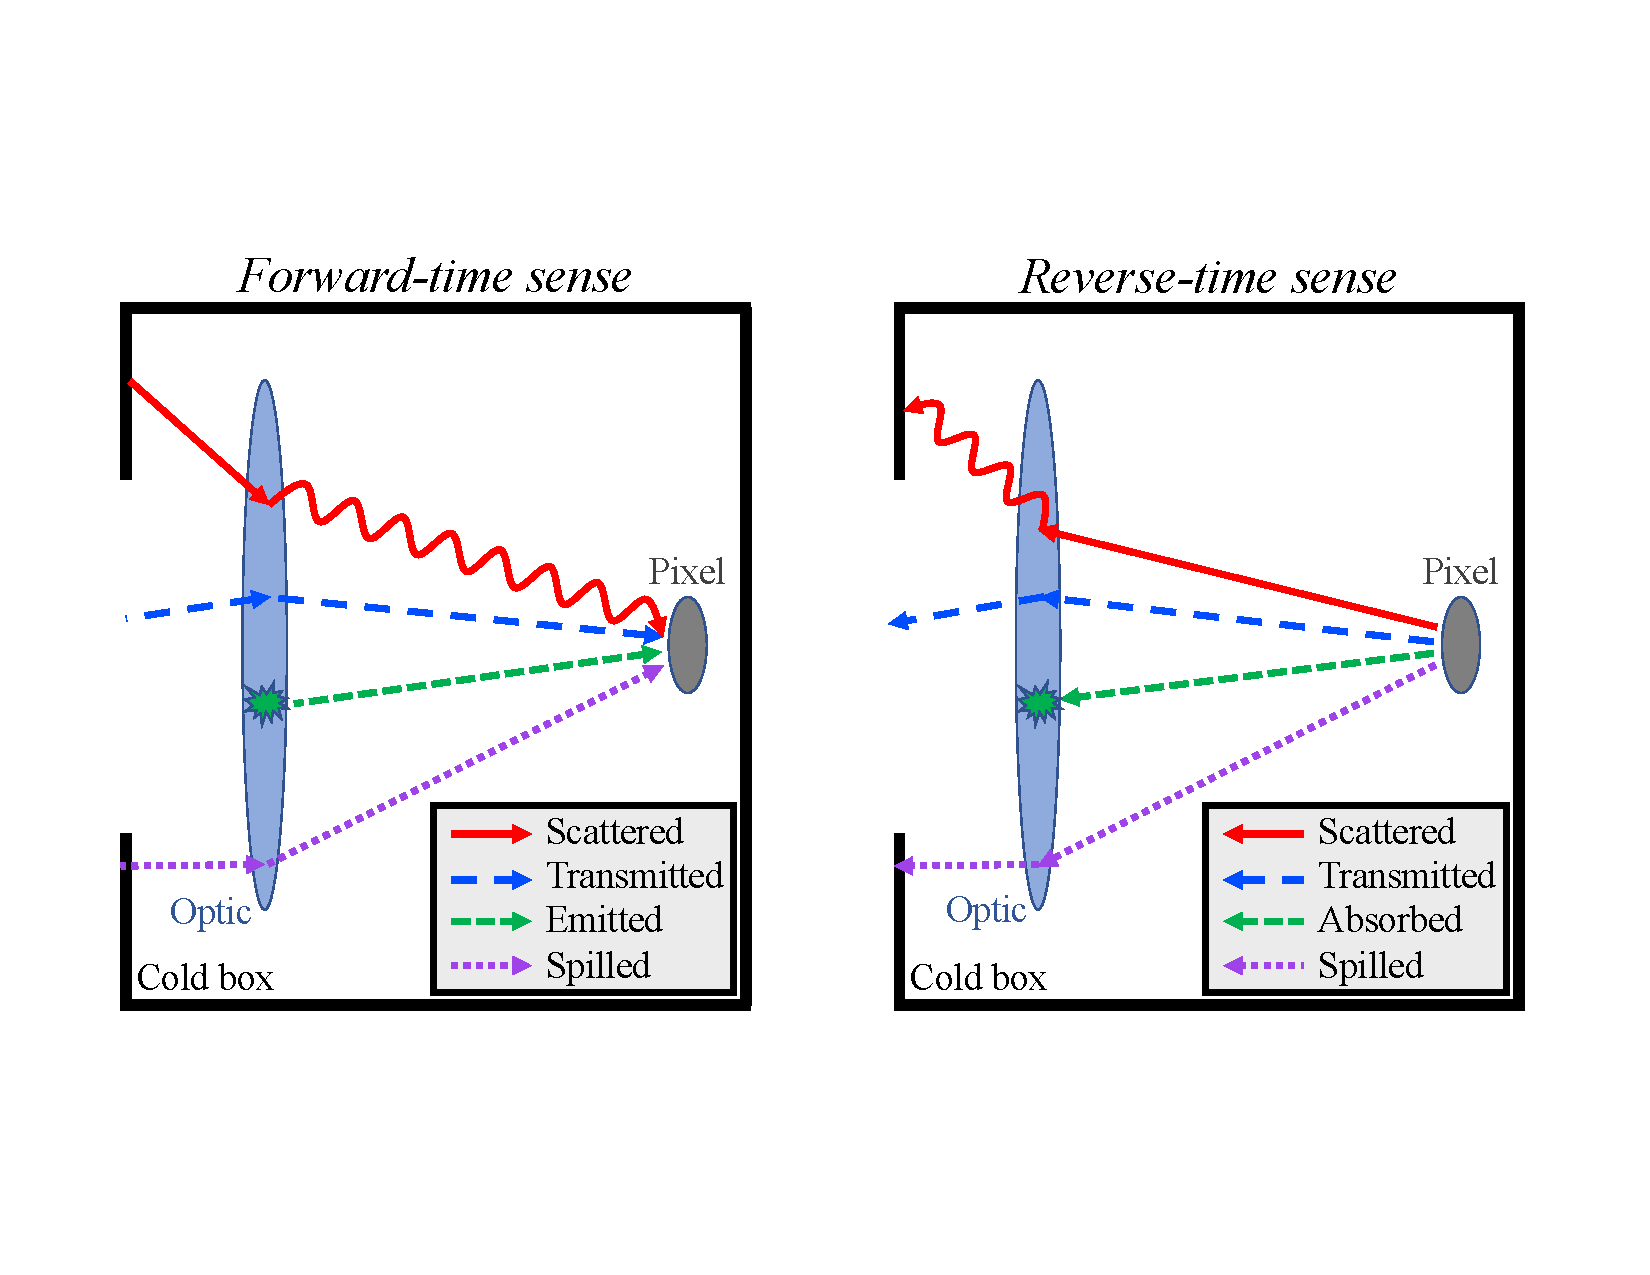
\includegraphics[width=\linewidth, trim=2cm 4cm 2cm 4cm, clip]{SensitivityCalculation/Figures/reverse_time_sense.pdf}
    \caption{A schematic to visually demonstrate the concept of reverse-time sense calculations as they apply to transmissivity, absorptivity/emissivity, scattering fraction, and spillover fraction. Most often when estimating sensitivities, it is useful to think in the reverse-time sense, or in the paradigm of the detector pixel emitting towards the sky.}
    \label{fig:reverse_time_sense}
\end{figure}

Assume that the optical stack, which comprises the telescope's mirrors, the receiver's lenses and filters, and the focal plane's optics, can be represented as a one-dimensional array of blackbody absorbers/emitters/attenuators in thermal equilibrium. While such a situation is not in general true, as temperature gradients develop across optics and IR loads and fridge performance vary in time, it is a reasonable approximation for the NET calculation, which is a white-noise estimate. There are four primary components to the optical load on the detector, and for each, it is most useful to think in the time-reverse sense.

%%%%%%%%%%%%%%%%%%%%%%%%%%%%%%%%
%%%%%%%%%%%%%%%%%%%%%%%%%%%%%%%%

\subsection{Emissivity and absorptivity}
\label{sec:sensitivity_emissivity}

\important{Emissivity} is the propensity of an optical element to emit mm-wave radiation. For dielectrics, the emissivity is determined by its loss tangent
\begin{equation}
    \tan \delta = \frac{2 \pi \nu \varepsilon'' + \sigma}{2 \pi \omega \varepsilon'} \approx \frac{\varepsilon''}{\varepsilon'} \, ,
    \label{eq:loss_tangent}
\end{equation}
where $\sigma$ is the conductivity, the dielectric constant is
\begin{equation}
    \varepsilon = \varepsilon' - i \varepsilon'' \, ,
    \label{eq:dielectric_constant}
\end{equation}
and the approximation applies for low-loss materials where $\varepsilon'' \ll \varepsilon'$. The emissivity of the dielectric can then be written as
\begin{equation}
    \epsilon_{\mathrm{diel}}(\nu) = 1 - \exp \left( - \frac{2 \pi \nu n t}{c} \tan \delta \right) \approx -\frac{2 \pi \nu t}{c} \tan \delta \, ,
    \label{eq:dielectric_emissivity}
\end{equation}
where $t$ is the optical thickness, $c$ is the speed of light in a vacuum, $n$ is the refractive index of the dielectric, and the approximation applies in the limit of a small loss tangent.

For conductors, such as mirrors, emissivity is generated by Ohmic losses
\begin{equation}
    \epsilon_{\mathrm{cond}}(\nu) = 1 - 4 \sqrt{\frac{\pi \nu \mu_{0}}{\sigma}} \, ,
    \label{eq:ohmic_loss_emissivity}
\end{equation}
where $\sigma$ is the conductivity and $\mu_{0}$ is the permeability of free space. Note that this equation assumes normal incidence, and at oblique angles, conductors skin depth is different for the S and P polarizations, which gives rise to slight differences in emissivities for different polarizations. While such small effects are indeed an important systematic effect for an accurate extraction of CMB polarization fluctuations, they are not important for sensitivity, which is concerned with spatially and polarization-averaged loading estimates.

Under the assumption that each optical element is a blackbody, its emission results from the thermodynamic motions of its composing molecules, which are Gaussian random and wide-band (as opposed to more complex materials with feature-filled emission spectra). In this paradigm, it is a very good assumption that the emissivity and absorptivity are equivalent
\begin{equation}
    \alpha(\nu) \equiv \frac{P_{\mathrm{abs}}}{P_{\mathrm{in}}} = \epsilon(\nu) \, .
    \label{eq:emissivity_absorptivity_equivalence}
\end{equation}
Therefore, not only does dielectric emission lead to parasitic loading, but it also leads to signal attenuation.

%%%%%%%%%%%%%%%%%%%%%%%%%%%%%%%%
%%%%%%%%%%%%%%%%%%%%%%%%%%%%%%%%

\subsection{Spillover fraction}
\label{sec:sensitivity_spillover_fraction}

\important{Spillover fraction} is the fraction of incident power that spills over the diffraction-limited area of a given optical element
\begin{equation}
    \beta(\nu) \equiv \frac{P_{\mathrm{spill}}(\nu)}{P_{\mathrm{in}}(\nu)} \, ,
    \label{eq:spillover_fraction_definition}
\end{equation}
where again, $P_{\mathrm{in}}(\nu)$ and $P_{\mathrm{spill}}(\nu)$ are in general frequency-dependent. Spillover fraction is most easily imagined in the reverse-time sense, from the perspective of the detector radiating towards the sky. If some power from a given pixel falls outside the ``imaged'' region of any optical element, this radiation will not propagate to the sky but will instead terminate somewhere else. Given that the detector can ``see'' these non-optical regions, then, flipping into the forward time sense, photons emitted from these non-optical regions are detected, which gives rise to optical power on the bolometer. 

The intensity of the spillover radiation is in turn governed by the \important{effective temperature of the spillover radiation} $T_{\beta}$. Often times in CMB experiments, when radiation spills over an optic (in the reverse-time sense), it ``lands'' on some surface. For example, if the spill is over the Lyot, that surface would be the stop, or if the spill is over a lens, that surface would be somewhere in the cryostat, or if the spill is over the primary mirror, that surface could be either the sky or the ground. The aggregate radiation from these surfaces is most conveniently described by an \textit{effective temperature}, which is often defined as
\begin{equation}
    T_{\mathrm{eff}} \equiv \varepsilon_{\mathrm{surface}} T_{\mathrm{surface}} \, ,
    \label{eq:effective temperature}
\end{equation}
where $T_{\mathrm{surface}}$ the surface's physical temperature and $\varepsilon$ is its emissivity. The astute reader will note that plugging $T_{\mathrm{eff}}$ into the Planck spectrum is not the same as using the spectrum for $T_{\mathrm{phys}}$ modified by the emissivity $\varepsilon{\mathrm{surface}}$. However, the equivalence is sufficient in the Rayleigh-Jeans limit, which often suffices for the CMB instrument calculations to follow.

%%%%%%%%%%%%%%%%%%%%%%%%%%%%%%%%
%%%%%%%%%%%%%%%%%%%%%%%%%%%%%%%%

\subsection{Scattering fraction}
\label{sec:sensitivity_scattering_fraction}

\important{Scattering fraction} is the fraction of incident power that is scattered by a given optical element
\begin{equation}
    \delta(\nu) \equiv \frac{P_{\mathrm{scatt}}(\nu)}{P_{\mathrm{in}}(\nu)} \, .
    \label{eq:scattering_fraction_definition}
\end{equation}
In a similar sense to spillover, scattering fraction is most easily imagined in the reverse-time sense, from the perspective of the detector radiating towards the sky. If some power from a given pixel is scattered by an optical element, this radiation will not propagate to the sky but will instead terminate onto some surface that will, in the forward-time sense, emit optical power on the bolometer. The intensity of the scattered radiation is also governed by the \important{effective temperature of the scattered radiation} $T_{\delta}$ and therefore also follows Equation~\ref{eq:effective temperature}.

There are many mechanisms for scattering, but the two most common in mm-wave experiments are Mie scattering and Ruze scattering. Mie scattering arises due to any irregularity in an otherwise homogeneous (or well-ordered) medium. Common examples in CMB telescopes are voids in dielectric substrates, air bubbles/gaps between anti-reflection coating layers, and sub-wavelength filler materials. In the limit that the scattering center is much smaller than the wavelength, which is often a good approximation in mm-wave telescopes, the Mie scattering is well-described by the Rayleigh scattering cross section
\begin{equation}
    \sigma_{\mathrm{Ray}} \equiv \frac{2 \pi^{5}}{3} \frac{d^{6}}{\lambda^{4}} \left( \frac{n_{2}^{2} - n_{1}^{2}}{n_{2}^{2} + 2 n_{1}^{2}} \right)^{2} \, ,
    \label{eq:rayleigh_scattering_cross_section}
\end{equation}
where $d$ is the diameter of the particle/void/deformity, $n_{2}$ is its refractive index, and $n_{1}$ is the refractive index of the medium. The aggregate impact of Rayleigh scatterers is then given by the Beer-Lambert Law
\begin{equation}
    \beta(\nu) = 1 - \exp \left( - \sigma_{\mathrm{Ray}} N z \right) \, ,
    \label{eq:beer_lambert_law}
\end{equation}
where $N$ is the number density of scatterers and $z$ is the optical path length of the scattering medium. Scattering is also a very important sensitivity parameter to calculate, characterize, and understand, especially because it does not improve with decreasing temperature, unlike dielectric loss.

Scattering from reflectors is typically due to their surface roughness and is quantified by Ruze scattering
\begin{equation}
    \beta_{\mathrm{Ruze}}(\nu) = 1 - \exp \left[ \left( \frac{4 \pi \sigma \nu}{c} \right)^{2} \right] \, ,
    \label{eq:ruze_scattering}
\end{equation}
where here $\sigma$ is the RMS roughness. At millimeter wavelengths, Ruze scattering tends to be small and therefore negligible for terrestrial experiments, but the impact of reflector scattering on sensitivity can be more prominent for low-load environments, such as in outer space, and can be an important factor when specifying mirror finishes.

%%%%%%%%%%%%%%%%%%%%%%%%%%%%%%%%
%%%%%%%%%%%%%%%%%%%%%%%%%%%%%%%%

\subsection{Reflectivity}
\label{sec:sensitivity_reflectivity}

\important{Reflectivity} is the fraction of incident power that is reflected away from any dielectric optic
\begin{equation}
    r(\nu) \equiv \frac{P_{\mathrm{refl}}(\nu)}{P_{\mathrm{in}}(\nu)} \, ,
    \label{eq:reflectivity_definition}
\end{equation}
Reflections arise at interfaces between media with different refractive indexes, and anti-reflection coatings are designed to limit these reflections. An in-depth discussion of AR coatings and their realized reflectivities is presented in Chapter~blah.

%%%%%%%%%%%%%%%%%%%%%%%%%%%%%%%%
%%%%%%%%%%%%%%%%%%%%%%%%%%%%%%%%

\subsection{Transmissivity}
\label{sec:sensitivity_reflectivity}

\important{Transmissivity} is the ratio of transmitted optical power to incident optical power
\begin{equation}
    \eta(\nu) \equiv \frac{P_{\mathrm{trans}}(\nu)}{P_{\mathrm{in}}(\nu)} \, ,
    \label{eq:transmissivity_definition}
\end{equation}
and is the product of absorptivity, spillover fraction, scattering fraction, and reflectivity
\begin{equation}
    \eta(\nu) = \left[ 1 - \alpha(\nu) \right] \left[ 1 - \beta(\nu) \right] \left[ 1 - \delta(\nu) \right] \left[ 1 - r(\nu) \right] \, .
    \label{eq:transmissivity_product}
\end{equation}
Transmissivity is effectively synonymous with transparency, and maximizing it is a core principle of high-throughput telescopes.

%%%%%%%%%%%%%%%%%%%%%%%%%%%%%%%%
%%%%%%%%%%%%%%%%%%%%%%%%%%%%%%%%

\subsection{Optical throughput and optical efficiency}
\label{sec:sensitivity_optical_throughput_optical_efficiency}

The \important{optical throughput} of the instrument is defined to be the total transmission through all optical elements in the telescope + camera, including the detector, and is defined as
\begin{equation}
    \eta_{\mathrm{through}} = \prod_{i=0}^{N_{\mathrm{inst}}} \eta_{i}
    \label{eq:throughput}
\end{equation}
where $N_{\mathrm{inst}}$ represents all optical elements within in the instrument and excludes the atmosphere. As noted in Section~\ref{sec:focal_plane_optics}, the aperture stop (or the Lyot stop in telescopes with reimaging optics) defines the angular resolution of the telescope and therefore truncates the beam from the detector pixels, leading to an an efficiency loss. Unlike other transmissivity degradations, that of the aperture is intentional, and therefore it is common to quote the \important{optical efficiency} of an instrument
\begin{equation}
    \eta_{\mathrm{eff}} = \frac{\eta_{\mathrm{through}}}{\eta_{\mathrm{apert}}} \, ,
    \label{eq:optical_efficiency}
\end{equation}
where $\eta_{\mathrm{apert}}$ is the aperture efficiency (also called the beam-coupling efficiency) defined in Equation~\ref{eq:beam_coupling_efficiency}. The theoretical maximum of $\eta_{\mathrm{eff}}$, in the limit of a perfectly transparent optical stack, is 100\%, while that of $\eta_{\mathrm{through}}$ is $1 - \eta_{\mathrm{apert}}$.

%%%%%%%%%%%%%%%%%%%%%%%%%%%%%%%%
%%%%%%%%%%%%%%%%%%%%%%%%%%%%%%%%

\subsection{Sky temperature and telescope temperature}
\label{sec:sensitivity_telescope_temperature_sky_temperature}

In the broadest sense, there are two ``sources'' of optical loading on the bolometer: the sky and the instrument
\begin{equation}
    P_{\mathrm{opt}} = P_{\mathrm{sky}} + P_{\mathrm{inst}} \, .
    \label{eq:sky_and_instrument_power}
\end{equation}
Here, sky power is given by
\begin{equation}
    P_{\mathrm{sky}} = \int_{0}^{\infty} \left[ \sum_{i}^{N_{\mathrm{sky}}} p_{i} (\nu) \right] B (\nu) \mathrm{d} \nu \, ,
    \label{eq:sky_power}
\end{equation}
where the summation runs over all $N_{\mathrm{sky}}$ sky sources, including the CMB, galactic dust emission, synchrotron emission, and atmospheric emission. In a similar manner, and instrument power is given by
\begin{equation}
    P_{\mathrm{inst}} = \int_{0}^{\infty} \left[ \sum_{i}^{N_{\mathrm{inst}}} p_{i} (\nu) \right] B (\nu) \mathrm{d} \nu \, ,
    \label{eq:inst_pow}
\end{equation}
where the summation runs over all $N_{\mathrm{inst}}$ instrument sources, such as the telescope mirrors, vacuum window, lenses, thermal filters, aperture stop, and focal plane coupling optics. 

Given the partition of the optical power on the detector into that due to the sky and that due to the instrument, it is common practice to describe each load in terms of an effective temperature
\begin{equation}
    P_{\mathrm{opt}} = \eta_{\mathrm{inst}} k_{\mathrm{B}} \Delta \nu \left( T_{\mathrm{sky}} + T_{\mathrm{inst}} \right) \, ,
    \label{eq:telescope_temperature_sky_temperature}
\end{equation}
where $\Delta \nu$ is the effective bandwidth, which is typically defined as the distance between the detector band's $B(\nu)$ -3~dB points. Equation~\ref{eq:telescope_temperature_sky_temperature} essentially describes the total power from the sky and the telescope as being due to a perfect blackbody placed in front of a 0~K telescope with efficiency $\eta_{\mathrm{inst}}$. This scheme allows parasitic power for telescope optics to be quickly compared against that of the sky, which is often useful during instrument design and characterization as a major goal of the instrument design to make $T_{\mathrm{tel}} < T_{\mathrm{sky}}$.

%%%%%%%%%%%%%%%%%%%%%%%%%%%%%%%%
%%%%%%%%%%%%%%%%%%%%%%%%%%%%%%%%
%%%%%%%%%%%%%%%%%%%%%%%%%%%%%%%%

\section{Bolometer thermal carrier NEP}
\label{sec:bolometer_thermal_carrier_noise}

Bolometer thermal carrier noise arises due to fluctuations in heat flow between the absorbing element and the bath to which it is weakly connected and is given by the equation
\begin{equation}
    NEP_{\mathrm{g}} = \sqrt{4 k_{\mathrm{B}} F_{\mathrm{link}} T_{\mathrm{c}}^{2} g}\, ,
    \label{eq:nep_g}
\end{equation}
where $T_{\mathrm{c}}$ is the bolometer operating temperature (which for a TES is equivalent to its superconducting transition temperature), $G$ is the thermal conductance from the absorbing element to the bath, and $F_{\mathrm{link}}$ is a numerical factor that depends on the link's thermal conduction index $n$
\begin{equation}
    F_{\mathrm{link}} = \frac{\int_{T_{\mathrm{b}}}^{T_{\mathrm{c}}} \left[ \frac{T k(T)}{T_{\mathrm{c}} k(T_{\mathrm{c}})} \right]^{2} \dd T}{\int_{T_{\mathrm{b}}}^{T_{\mathrm{c}}} \left[ \frac{k(T)}{k(T_{\mathrm{c}})} \right] \dd T} = \frac{n + 1}{2 n + 3} \frac{1 - \left( T_{\mathrm{b}} / T_{\mathrm{c}} \right)^{2n + 3}}{1 - \left( T_{\mathrm{b}} / T_{\mathrm{c}} \right)^{n + 1}} \, ,
    \label{eq:flink}
\end{equation}
where $T_{\mathrm{b}}$ is the bath temperature and where the conductivity between the bolometer and the bath is assumed to be $k(T) = k_{0} T^{n}$.

\begin{figure}
    \centering
    \subfloat[\label{fig:nepg_vs_Tc:a}]{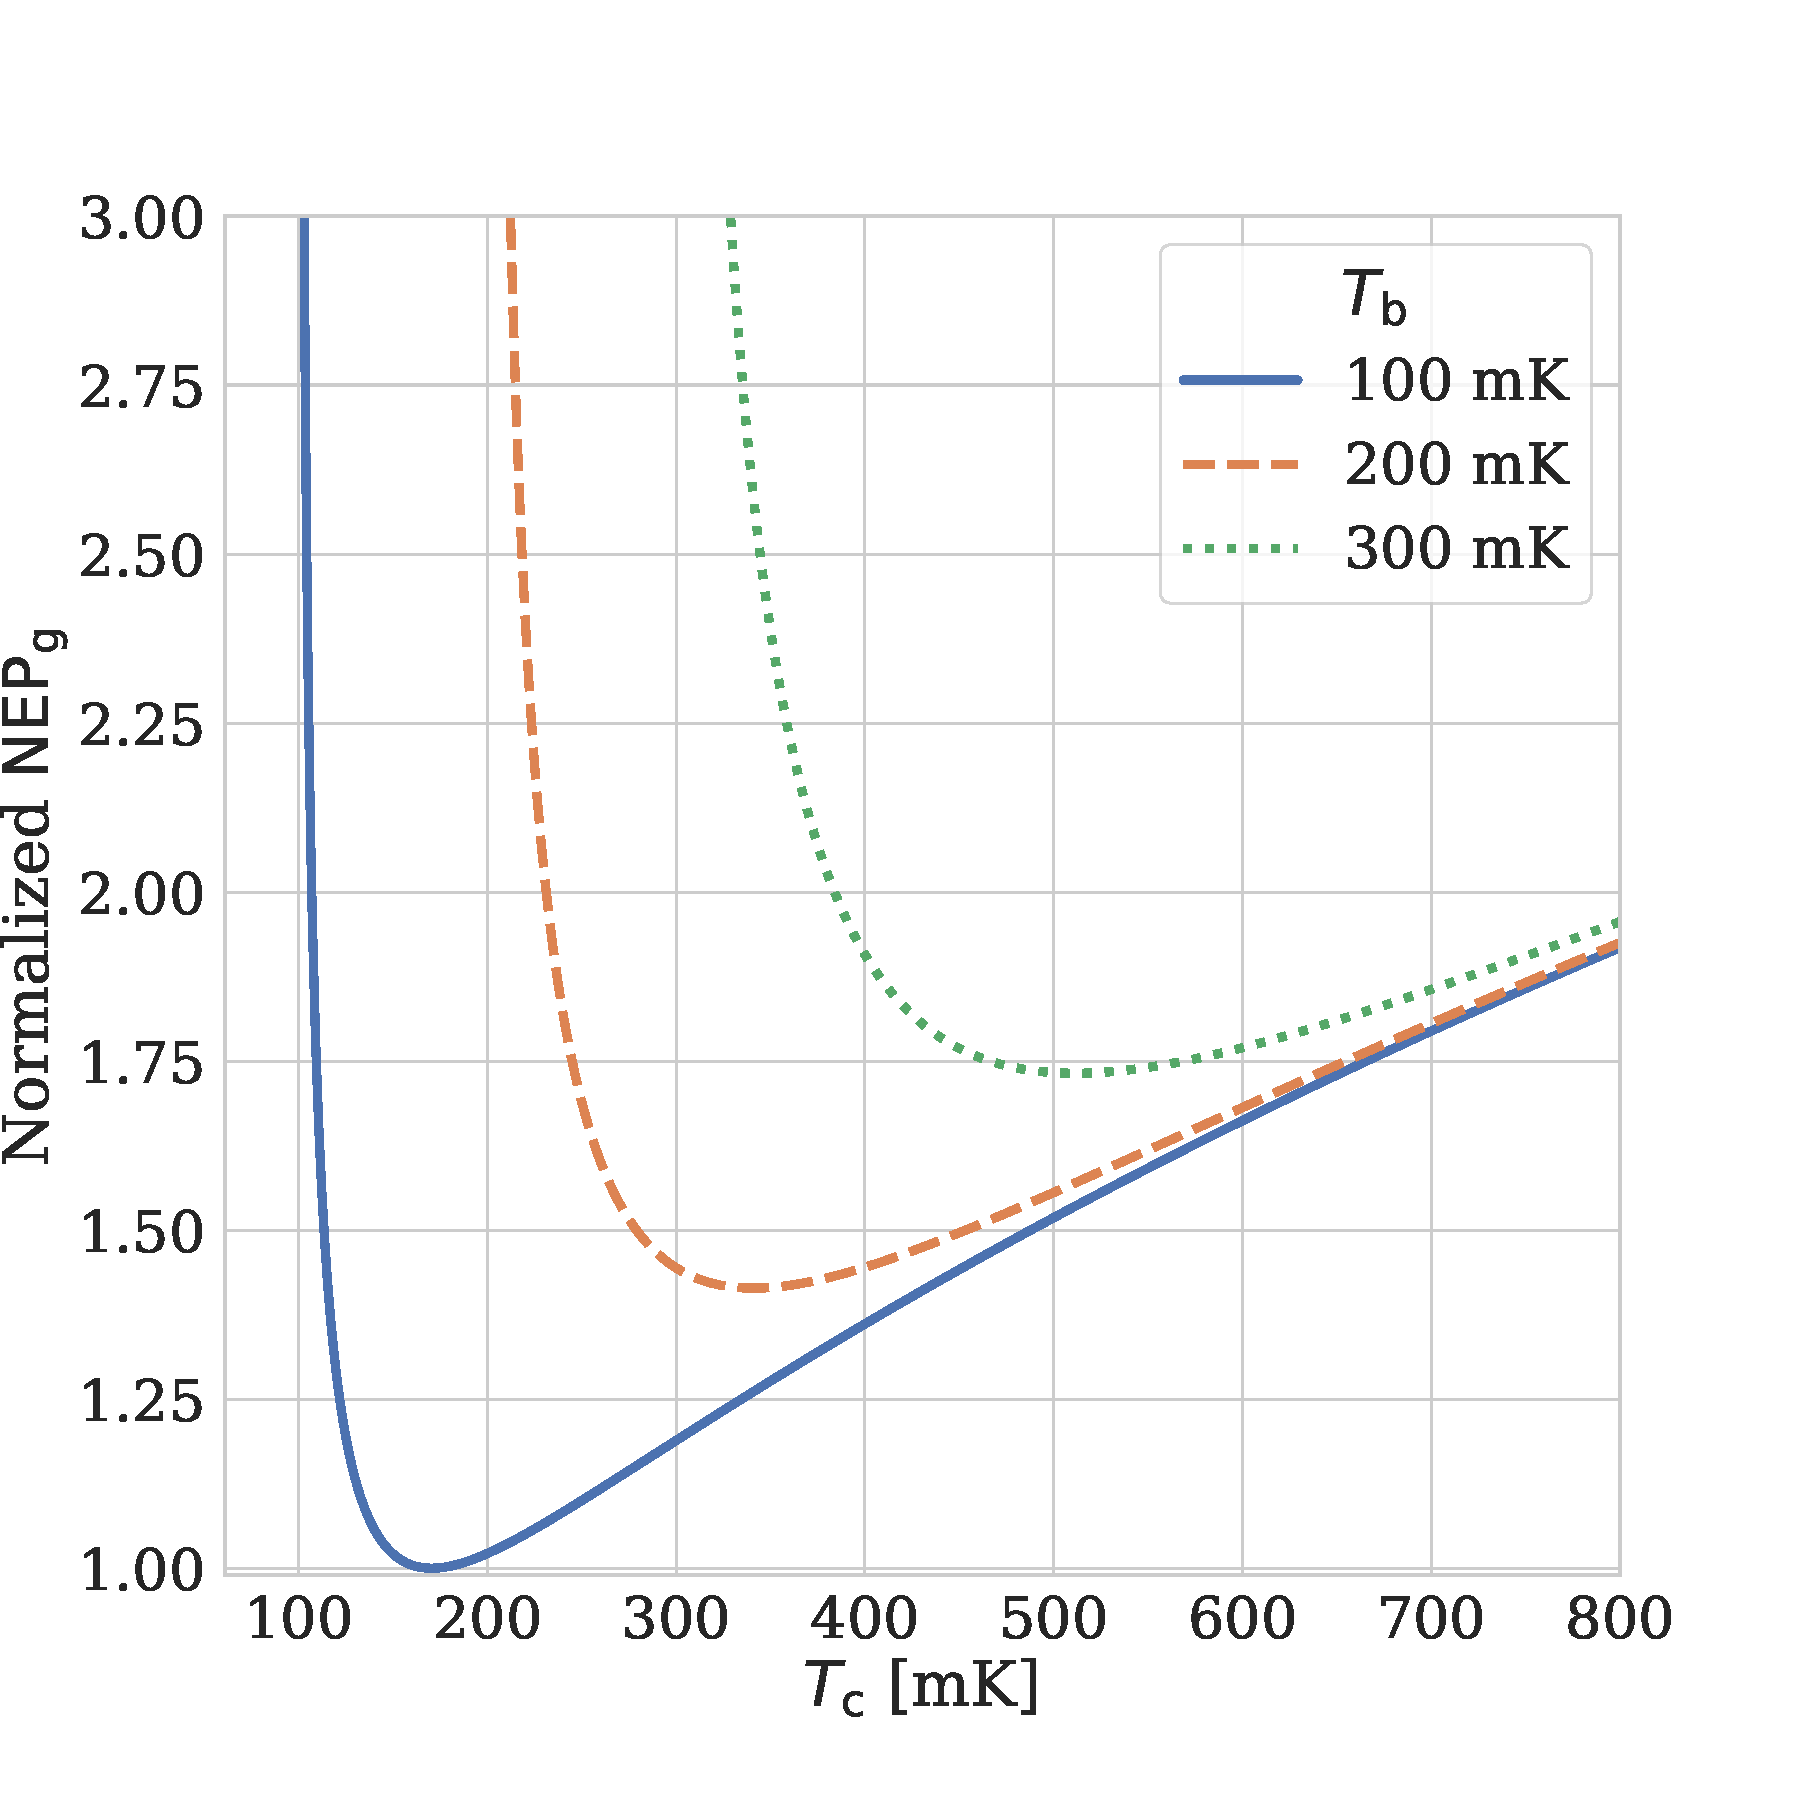
\includegraphics[width=0.48\linewidth, trim=0cm 1cm 2cm 3cm, clip]{SensitivityCalculation/Figures/NEPg_vs_Tc.pdf}}
    \subfloat[\label{fig:nepg_vs_Tc:b}]{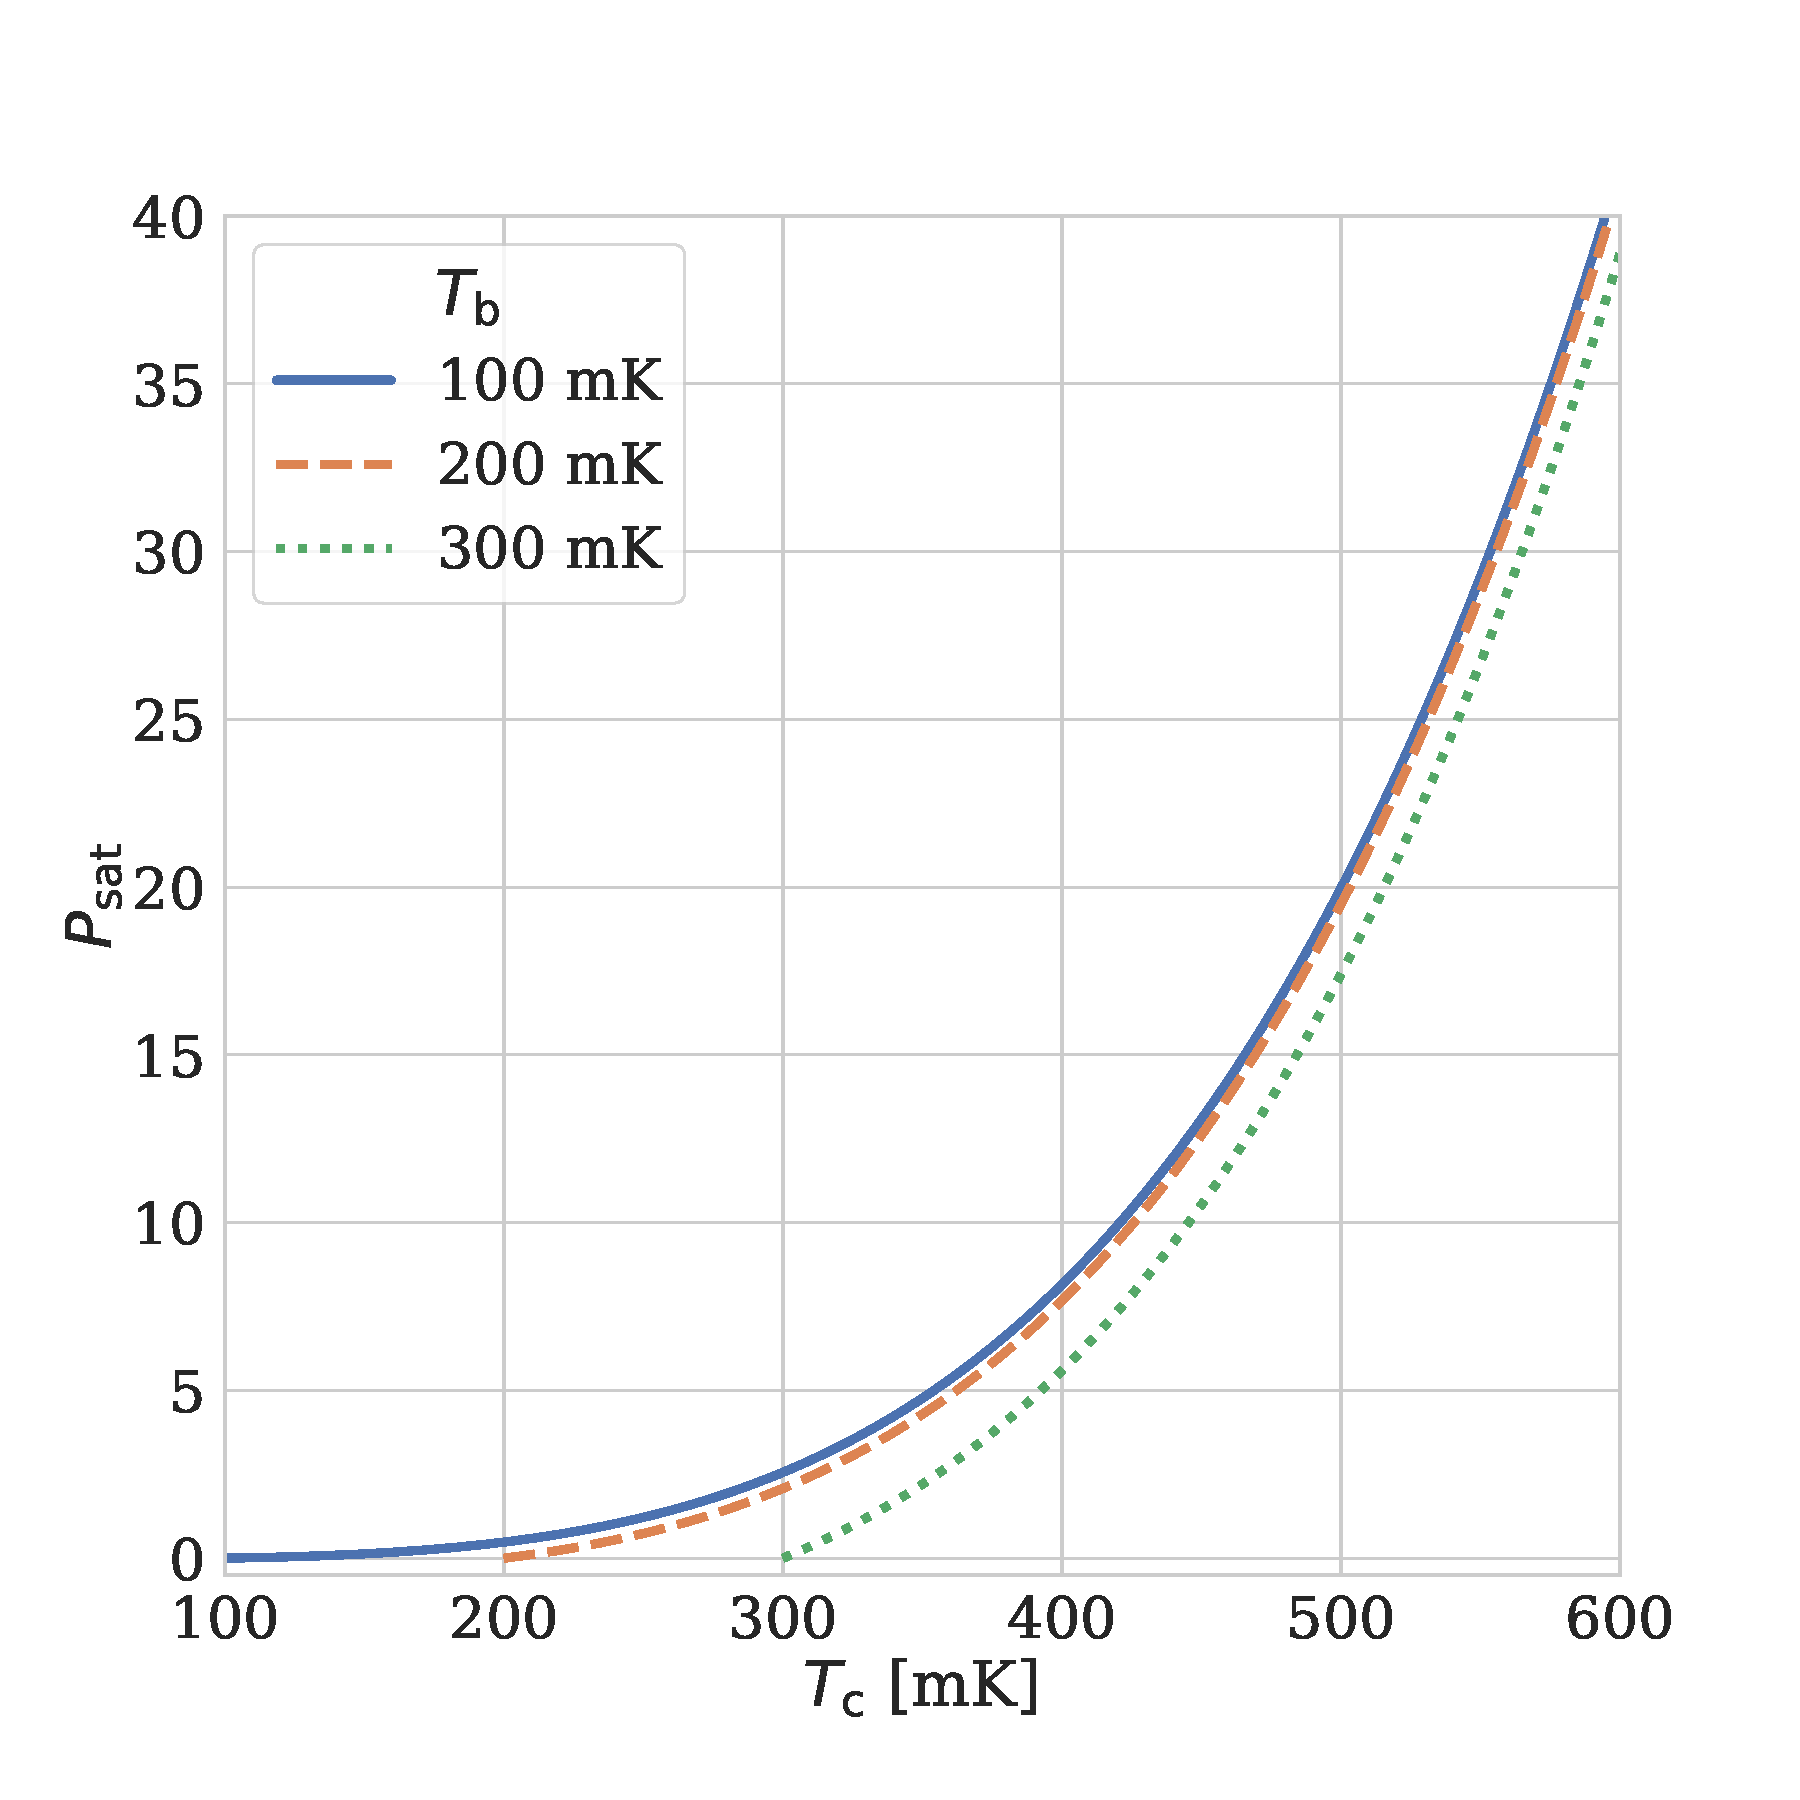
\includegraphics[width=0.48\linewidth, trim=0cm 1cm 2cm 3cm, clip]{SensitivityCalculation/Figures/Psat_vs_Tc.pdf}}
    \caption{Dependence of (a) $\mathrm{NEP_{g}}$ and (b) $P_{\mathrm{sat}}$ on bolometer transition temperature $T_{\mathrm{c}}$ for various bath temperatures $T_{\mathrm{b}}$. (a) assumes a constant $P_{\mathrm{sat}}$, and (b) assumes $A k_{0} / (n + 1) = 240$~$\mathrm{pW / mm \; K^{4}}$ and a bolometer ``leg'' length of 1~mm. Reducing bath temperature substantially improves thermal carrier noise while having little impact on saturation power. For a given $T_{\mathrm{b}}$, there optimum transition temperature is $T_{\mathrm{c}} \approx 1.7 T_{\mathrm{b}}$.}
    \label{fig:nepg_vs_Tc}
\end{figure}

The power flowing from the bolometer to the thermal bath is given by
\begin{equation}
    P_{\mathrm{sat}} = \int_{T_{\mathrm{b}}}^{T_{\mathrm{c}}} \frac{A}{l} k(T) \dd T = \frac{A}{l} \frac{k_{0}}{(n + 1)} \left( T_{\mathrm{c}}^{n + 1} - T_{\mathrm{b}}^{n + 1} \right)
    \label{eq:saturation_power_conductivity}
\end{equation}
where $A$ and $l$ are the cross sectional area and length, respectively, of the link between the TES and the thermal bath. We can then calculate the dynamic thermal conductance as
\begin{equation}
    g = \frac{\partial P_{\mathrm{sat}}}{\partial T} = \frac{A}{l} k_{0} T_{\mathrm{c}}^{n} \, .
    \label{eq:dynamic_conductance_a_over_l}
\end{equation}
While the details of the bolometer thermal link are familiar to those that design and fabricate bolometers, saturation power is typically what's measured, and therefore it's useful to rewrite $g$ as
\begin{equation}
    g = P_{\mathrm{sat}} (n + 1) \frac{T_{\mathrm{c}}^{n}}{T_{\mathrm{c}}^{n+1} - T_{\mathrm{b}}^{n+1}}
    \label{eq:g}
\end{equation}
Therefore, $NEP_{\mathrm{g}} \propto P_{\mathrm{sat}}$, making the tuning of saturation power important to optimizing detector sensitivity. Plugging this conductance into Equation~\ref{eq:nep_g} gives a more phenomenological form for thermal carrier noise
\begin{equation}
    \mathrm{NEP_{g}} = \sqrt{4 k_{\mathrm{B}} F_{\mathrm{link}} P_{\mathrm{sat}}} \sqrt{\frac{\left(n + 1 \right) T_{\mathrm{c}}^{n + 2}}{T_{c}^{n+1} - T_{\mathrm{b}}^{n + 1}}} \, .
    \label{eq:nep_g_phenomenological}
\end{equation}
While Equation~\ref{eq:nep_g_phenomenological} is fully determined by a relatively small set of measurable quantities, in reality $NEP_{\mathrm{g}}$ can vary depending on the specifics of the bolometer geometry, composition and fabrication. For example, transition-edge sensors (TES) have known pathological noise sources, such as flux flow noise and non-equilibrium Johnson noise, that increase the measured $NEP_{\mathrm{g}}$ beyond that of the theoretical presented here. Therefore, $F_{\mathrm{link}}$ is often determined empirically during non-optical characterization both in the lab.

%%%%%%%%%%%%%%%%%%%%%%%%%%%%%%%%
%%%%%%%%%%%%%%%%%%%%%%%%%%%%%%%%
%%%%%%%%%%%%%%%%%%%%%%%%%%%%%%%%

\section{Readout NEP}
\label{sec:sensitivity_readout_noise}

As presented in Section~\ref{sec:simons_array_detectors}, modern CMB detectors are low-impedance, voltage-biased bolometers read out using superconducting quantum interference device (SQUID) transimpedance amplifiers. SQUIDs are current sensors, and a modulation of power on a voltage-biased bolometer corresponds to a modulation of current at the amplifier input. Therefore, SQUID amplifier noise is typically characterized in terms of a noise-equivalent current NEI, which has units of $\mathrm{A /\sqrt{Hz}}$. In order to refer NEI to an NEP, we need to consider the bolometer responsivity $S_{\mathrm{I}} = \mathrm{d} I / \mathrm{d} P$. One useful way to quantify responsivity is via the relation
\begin{equation}
    S_{\mathrm{I}} = -S_{\mathrm{fact}} \frac{1}{V_{\mathrm{elec}}}
    \label{eq:approx_responsivity}
\end{equation}
where $V_{\mathrm{bias}}$ is the bias voltage across the bolometer. In the presence of electrothermal feedback, the bolometer responsivity can typically be written in terms of the bolometer DC loop gain $\mathcal{L}$, the bolometer time constant $\tau$, and the modulation mode frequency $\omega$ as
\begin{equation}
    S_{\mathrm{fact}} = -\tilde{S}_{\mathrm{fact}} \frac{\mathcal{L}}{\mathcal{L} + 1} \frac{1}{1 + i \omega \tau}
    \label{eq:responsivity}
\end{equation}
where $\tilde{S}_{\mathrm{fact}}$ is 1 if $V_{\mathrm{bias}}$ is DC (e.g. time-division multiplexing or microwave multiplexing) or $\sqrt{2}$ if it is AC (frequency-domain multiplexing), as shown in Equation~\ref{eq:readout_responsivity}.

Characterization of the bolometer loop gain $\mathcal{L}$ and time constant $\tau$ are hugely important to determining detector responsivity and hence to correctly calibrating sky power in Watts to amplifier output in ADC counts. As a result, detector responsivity is calibrated frequently in the field using both celestial sources and instrumental techniques. Given an accurate estimate of $S_{\mathrm{fact}}$, \important{readout NEP} can be written as
\begin{equation}
    \mathrm{NEP}_{\mathrm{read}} = \frac{\mathrm{NEI}}{S_{\mathrm{I}}} = \frac{\sqrt{R_{\mathrm{bolo}} P_{\mathrm{bias}}}}{S_{\mathrm{fact}}} \mathrm{NEI} \, ,
    \label{eq:nep_read}
\end{equation}
where we the RMS voltage bias $V_{\mathrm{bias}} = \sqrt{R_{\mathrm{bolo}} P_{\mathrm{bias}}}$.

Readout noise can in general be a conglomeration of a multitude of noise sources and electrical effects, and therefore readout NEI is not synonymous with SQUID NEI. SQUIDs noise is, in general, quite low $\sim$~5~pA/$\mathrm{\sqrt{Hz}}$, while noise in dfMUX systems (which are used by SA) can range anywhere from 10~$\sim$~50~pA/$\mathrm{\sqrt{Hz}}$ and noise in $\mu$MUX systems (which are used by SO) can be even higher. An effective technique to suppress the conversion of these noise sources to power is to minimize $R_{\mathrm{bolo}}$. SO bolometers are DC biased and have a resistance of $\mathcal{O}(10)$~$\mathrm{m \Omega}$, while SA bolometers are AC biased, necessitating a larger resistance to minimize the impact of parasitic series impedances (such as, for example, inductance in the cables and connectors between the SQUID at 4~K and the detectors on mK stage), and have a resistance of $\mathcal{O}(1)$~$\Omega$. Minimizing readout noise a central pursuit of modern experiments, especially as they face the challenges associated with large multiplexing factors at high frequency.

%%%%%%%%%%%%%%%%%%%%%%%%%%%%%%%%
%%%%%%%%%%%%%%%%%%%%%%%%%%%%%%%%
%%%%%%%%%%%%%%%%%%%%%%%%%%%%%%%%

\section{Johnson NEP}
\label{sec:johnson_noise}

Johnson noise arises due to thermal fluctuations in the bolometer which in turn cause resistance fluctuations. Johnson noise equivalent current $\mathrm{NEI}_{\mathrm{johnson}}$ is given by
\begin{equation}
    \mathrm{NEI}_{\mathrm{johnson}} = \frac{1}{\mathcal{L}} \sqrt{\frac{4 k_{\mathrm{B}} T_{\mathrm{c}}}{R_{\mathrm{bolo}}}} \, ,
    \label{eq:nei_johnson}
\end{equation}
where again, $T_{\mathrm{c}}$ the bolometer's operating temperature and $R_{\mathrm{bolo}}$ is its operating resistance. Johnson current noise can be converted to an NEP using the bolometer responsivity $S_{\mathrm{I}}$, which is defined in Equation \ref{eq:responsivity} as
\begin{equation}
    \mathrm{NEP}_{\mathrm{johnson}} = \frac{\mathrm{NEI}_{\mathrm{johnson}}}{S_{\mathrm{I}}} = \tilde{S}_{\mathrm{fact}} \frac{\mathcal{L} + 1}{\mathcal{L}^{2}} \left( 1 + i \omega \tau \right) \sqrt{4 k_{\mathrm{B}} T_{\mathrm{c}} P_{\mathrm{bias}}} \:,
    \label{eq:nep_johnson}
\end{equation}
where $P_{\mathrm{bias}}$ is defined in Equation \ref{eq:p_elec}. 

Two important notes regarding Equation~\ref{eq:nep_johnson}. First, in the limit of large loop gain $\mathcal{L} \gg 1$, which is often achievable for TES bolometers due to their large $\dd R / \dd T$, $NEP_{\mathrm{johnson}} \rightarrow 0$. Second, Johnson noise is suppressed by a factor of factor of $1 / \mathcal{L}$ with respect to readout noise. For these two reasons, it is often customary to ignore Johnson noise when estimate the NEP of TESes. Even in a worse-possible-case scenario of $\mathcal{L} = 1$, the estimated $\mathrm{NEI_{Johnson}}$ for SA (SO) bolometer is $\sim$~5~(20)~$\mathrm{pA / \sqrt{Hz}}$, which is far below the $\mathrm{NEI_{readout}}$ values discussed in Section~\ref{sec:sensitivity_readout_noise}. This comparison becomes even starker when assuming a healthier, more typical loop gain of, for example, $\mathcal{L}$~$\sim$~10.

%%%%%%%%%%%%%%%%%%%%%%%%%%%%%%%%
%%%%%%%%%%%%%%%%%%%%%%%%%%%%%%%%
%%%%%%%%%%%%%%%%%%%%%%%%%%%%%%%%

\section{NET}
\label{sec:sensitivity_calculation_net}

Assuming that the all detector noise sources are white and uncorrelated, the total detector NEP is given as
\begin{equation}
    \mathrm{NEP}_{\mathrm{det}} = \sqrt{\mathrm{NEP}_{\mathrm{ph}}^{2} + \mathrm{NEP}_{\mathrm{g}}^{2} + \mathrm{NEP}_{\mathrm{read}}^{2}}
    \label{eq:nep_det}
\end{equation}
where $\mathrm{NEP}_{\mathrm{ph}}$ is the photon NEP, $\mathrm{NEP}_{\mathrm{g}}$ is the thermal carrier NEP, and $\mathrm{NEP}_{\mathrm{read}}$ is the readout NEP.

Because a bolometer is built to measure fluctuations in the incident power due to fluctuations in the sky temperature, it is useful to convert bolometer NEP into a noise-equivalent sky temperature (NET) 
\begin{equation}
    \mathrm{NET}_{\mathrm{det}} = \frac{\mathrm{NEP}_{\mathrm{det}}}{\sqrt{2} \left( \mathrm{d} P / \mathrm{d} T_{\mathrm{sky}} \right)}
    \label{eq:net}
\end{equation}
where the $\sqrt{2}$ arises due to a unit conversion from output bandwidth $1 / \sqrt{\mathrm{Hz}}$ to integration time $\sqrt{s}$.

\begin{figure}[!t]
    \centering
    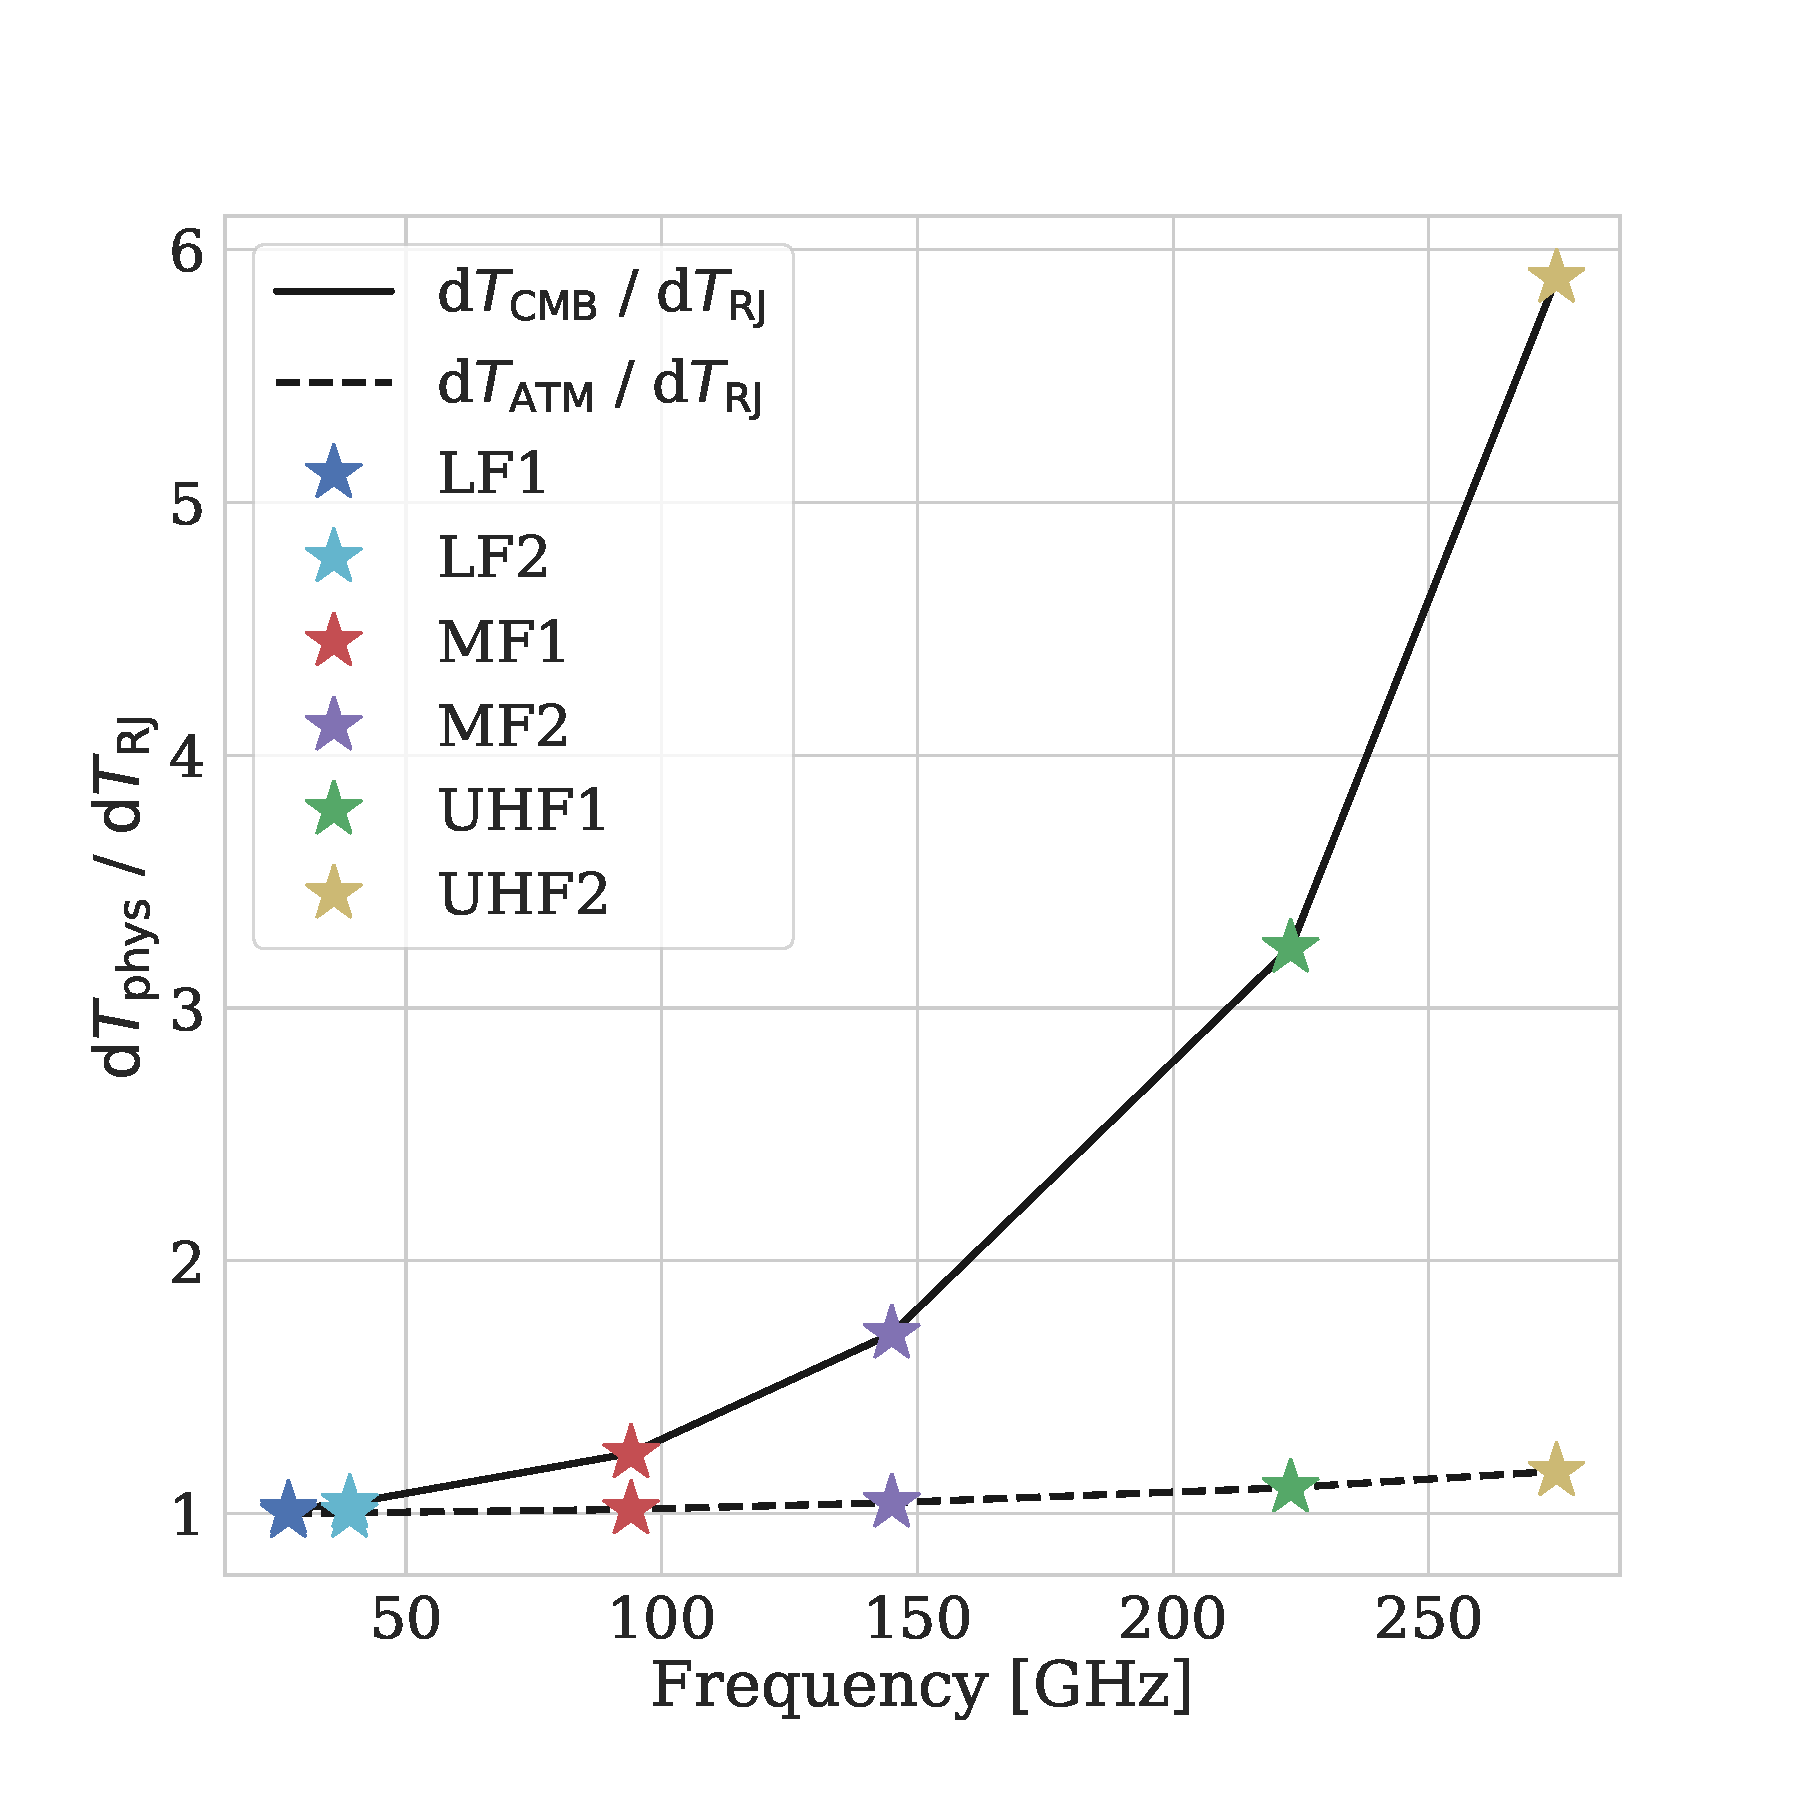
\includegraphics[width=0.6\linewidth, trim=1cm 1cm 1cm 3.5cm, clip]{SensitivityCalculation/Figures/dTcmb_dTrj_conversion.pdf}
    \caption{Conversion factor from RJ temperature fluctuations to that of a blackbody source with temperature $T_{\mathrm{phys}}$. The most commonly used factor is $\dd T_{\mathrm{CMB}} / \dd T_{\mathrm{RJ}}$, which is used to convert $\mathrm{NET_{RJ}}$ to $\mathrm{NET_{CMB}}$, but for reference, the conversion factor for a 10~K atmosphere is also plotted. These lines demonstrate that the Rayleigh-Jeans approximation works well for high temperatures and at low frequencies, and therefore it is often used to assess radio telescopes and IR telescopes that observe bright sources.}
    \label{fig:dTcmb_dTrj}
\end{figure}

CMB experiments often describe sky power referenced to either the CMB with physical temperature $T_{\mathrm{phys}} = T_{\mathrm{CMB}} = 2.725$~K or to some other source with Rayleigh-Jeans temperature $T_{\mathrm{RJ}}$. The conversion factor from fluctuations in the physical temperature of a blackbody with temperature $T_{\mathrm{phys}}$ to power is
\begin{equation}
    \frac{\mathrm{d} P}{\mathrm{d} T_{\mathrm{phys}}} = \xi \int_{0}^{\infty} \left[ \prod_{i=1}^{N_{\mathrm{elem}}} \frac{1}{k_{\mathrm{B}}} \left(  \frac{h \nu}{T_{\mathrm{phys}} \left( \exp \left[ h \nu / k_{\mathrm{B}} T_{\mathrm{phys}} \right] - 1 \right) } \right)^{2} \exp \left[h \nu / k_{\mathrm{B}} T_{\mathrm{phys}} \right] \right] B(\nu) \mathrm{d} \nu
    \label{eq:tcmb_fact}
\end{equation}
where $\xi$ is an overall signal degradation factor, which might be, for example, associated with poor far-field image formation at the focal plane, and $B(\nu)$ is the detector bandpass. The conversion factor for $\mathrm{K_{RJ}}$ is
\begin{equation}
    \frac{\mathrm{d} P}{\mathrm{d} T_{\mathrm{RJ}}} = \xi \int_{0}^{\infty} k_{\mathrm{B}} B(\nu) \mathrm{d} \nu
    \label{eq:trj_fact}
\end{equation}
where $B(\nu)$ is the detector bandpass. Note that Equation~\ref{eq:tcmb_fact} has units of $\mathrm{W / K_{CMB}}$ and that Equation~\ref{eq:trj_fact} has units of $\mathrm{W / K_{RJ}}$.

When reconstructing the sky during analysis, data from each detector are coadded in the map domain to improve signal to noise in the final map. To quantify this SNR increase in the time domain, we defined ``array NET'' as the inverse-variance-weighted average of the NETs of all yielded detectors within a given frequency channel
\begin{equation}
    \mathrm{NET}_{\mathrm{arr}} = \sqrt{\frac{1}{ \sum_{i}^{N_{\mathrm{det}}} 1 /  \mathrm{NET}_{i, \mathrm{det}}^{2}}} \Gamma \, ,
    \label{eq:net_inverse_variance_weight}
\end{equation}
where the sum is over all detectors in the array and where $\Gamma$ is a factor which quantifies the degree to which white noise is correlated between detector pixels on the focal plane (see Section~\ref{sec:sensitivity_calculation_correlation_factor} for more details). 

Equation~\ref{eq:net_inverse_variance_weight} is a useful estimate of aggregate NET as a common technique when combining data (across either multiple detectors or observations) is to weight the data by its inverse variance, to ensure that the highest SNR data is contributing the most power to the combined output. Under a simplifying assumption that all operational detectors have the same $\mathrm{NET_{det}}$, an assumption that is often invoked when forecasting \textit{median} sensitivity estimates, the inverse-variance weighted average becomes the simple average
\begin{equation}
    \mathrm{NET}_{\mathrm{arr}} = \frac{\mathrm{NET}_{\mathrm{det}}}{\sqrt{Y N_{\mathrm{det}}}} \Gamma
    \label{eq:net_arr}
\end{equation}
where $N_{\mathrm{det}}$ is the number of detectors in this frequency channel, $Y$ is the detector yield. Note that nonoperational detectors effectively have infinite $\mathrm{NET_{det}}$.

%%%%%%%%%%%%%%%%%%%%%%%%%%%%%%%%
%%%%%%%%%%%%%%%%%%%%%%%%%%%%%%%%
%%%%%%%%%%%%%%%%%%%%%%%%%%%%%%%%

\section{White-noise correlation factor}
\label{sec:sensitivity_calculation_correlation_factor}

It is possible to oversample the focal plane by deploying more detector pixels than there are non-overlapping spatial modes in the telescope optics. When the pixel density is higher than the mode density, Bose noise correlates between detector outputs. This slows the rate at which noise is averaged down during detector coaddition and is quantified in $\mathrm{NET_{arr}}$ via the factor $\Gamma$ in Equation~\ref{eq:net_arr}. A detailed derivation and discussion of white-noise correlations is discussed in Chapter~\ref{ch:white_noise_correlations}, but we briefly review the calculation here for the completeness of the sensitivity calculation presentation.

The number of optical modes in the telescope is determined by the sky beam size and by the field of view, and it is functionally synonymous with the number of non-overlapping telescope beams. For example, if the telescope's field of view is 5~deg and its beam size is 0.1~deg, the number of independent modes can be approximated as $(5 / 0.1)^{2}$. This description is rough and depends on the details of the beam profile and sidelobes, but this approximation is nonetheless intuitive and functional. In this paradigm, the telescope's magnification determines the linear dimension of the independent modes on the focal plane, which is $\approx 1.2$~$F \lambda$, as shown in Figure~blah. Therefore, if the detectors are packed more closely than $1.2$~$F \lambda$, their noise will start to correlate.

Intensity correlations are determined by the \important{Hanbury Brown-Twiss (HBT) coefficient}
\begin{equation}
    \gamma_{i,j} = \frac{\langle|e_{i}|^{2}|e_{j}|^{2}\rangle - \langle|e_{i}|^{2}\rangle\langle|e_{j}|^{2}\rangle}{\mathrm{RMS}\left(|e_{i}|^{2}\right) \, \mathrm{RMS}\left(|e_{j}|^{2}\right)} \, ,
\end{equation}
where $e_{i}$ is an integral of the electric field over the aperture for detector $i$ with beam $b_{i}(x,y)$ and optical path length to the source $\ell_{i}(x,y)$ 
\begin{equation}
    e_{i} = \iint \mathrm{d}x \, \mathrm{d}y \, e^{2 \pi i \ell_{i}(x,y)} \, b_{i}(x,y) \, E(x,y) \, .
\end{equation}
If the \textit{stop} is not 0~K, correlations can also arise due to radiation outside of the aperture as well. Again, these details are discussed in greater detail in Chapter~\ref{ch:white_noise_correlations}, but for now we focus only radiation within the aperture, which is typically the dominant noise contributor, especially for ground-based telescopes.

\begin{figure}
    \centering
    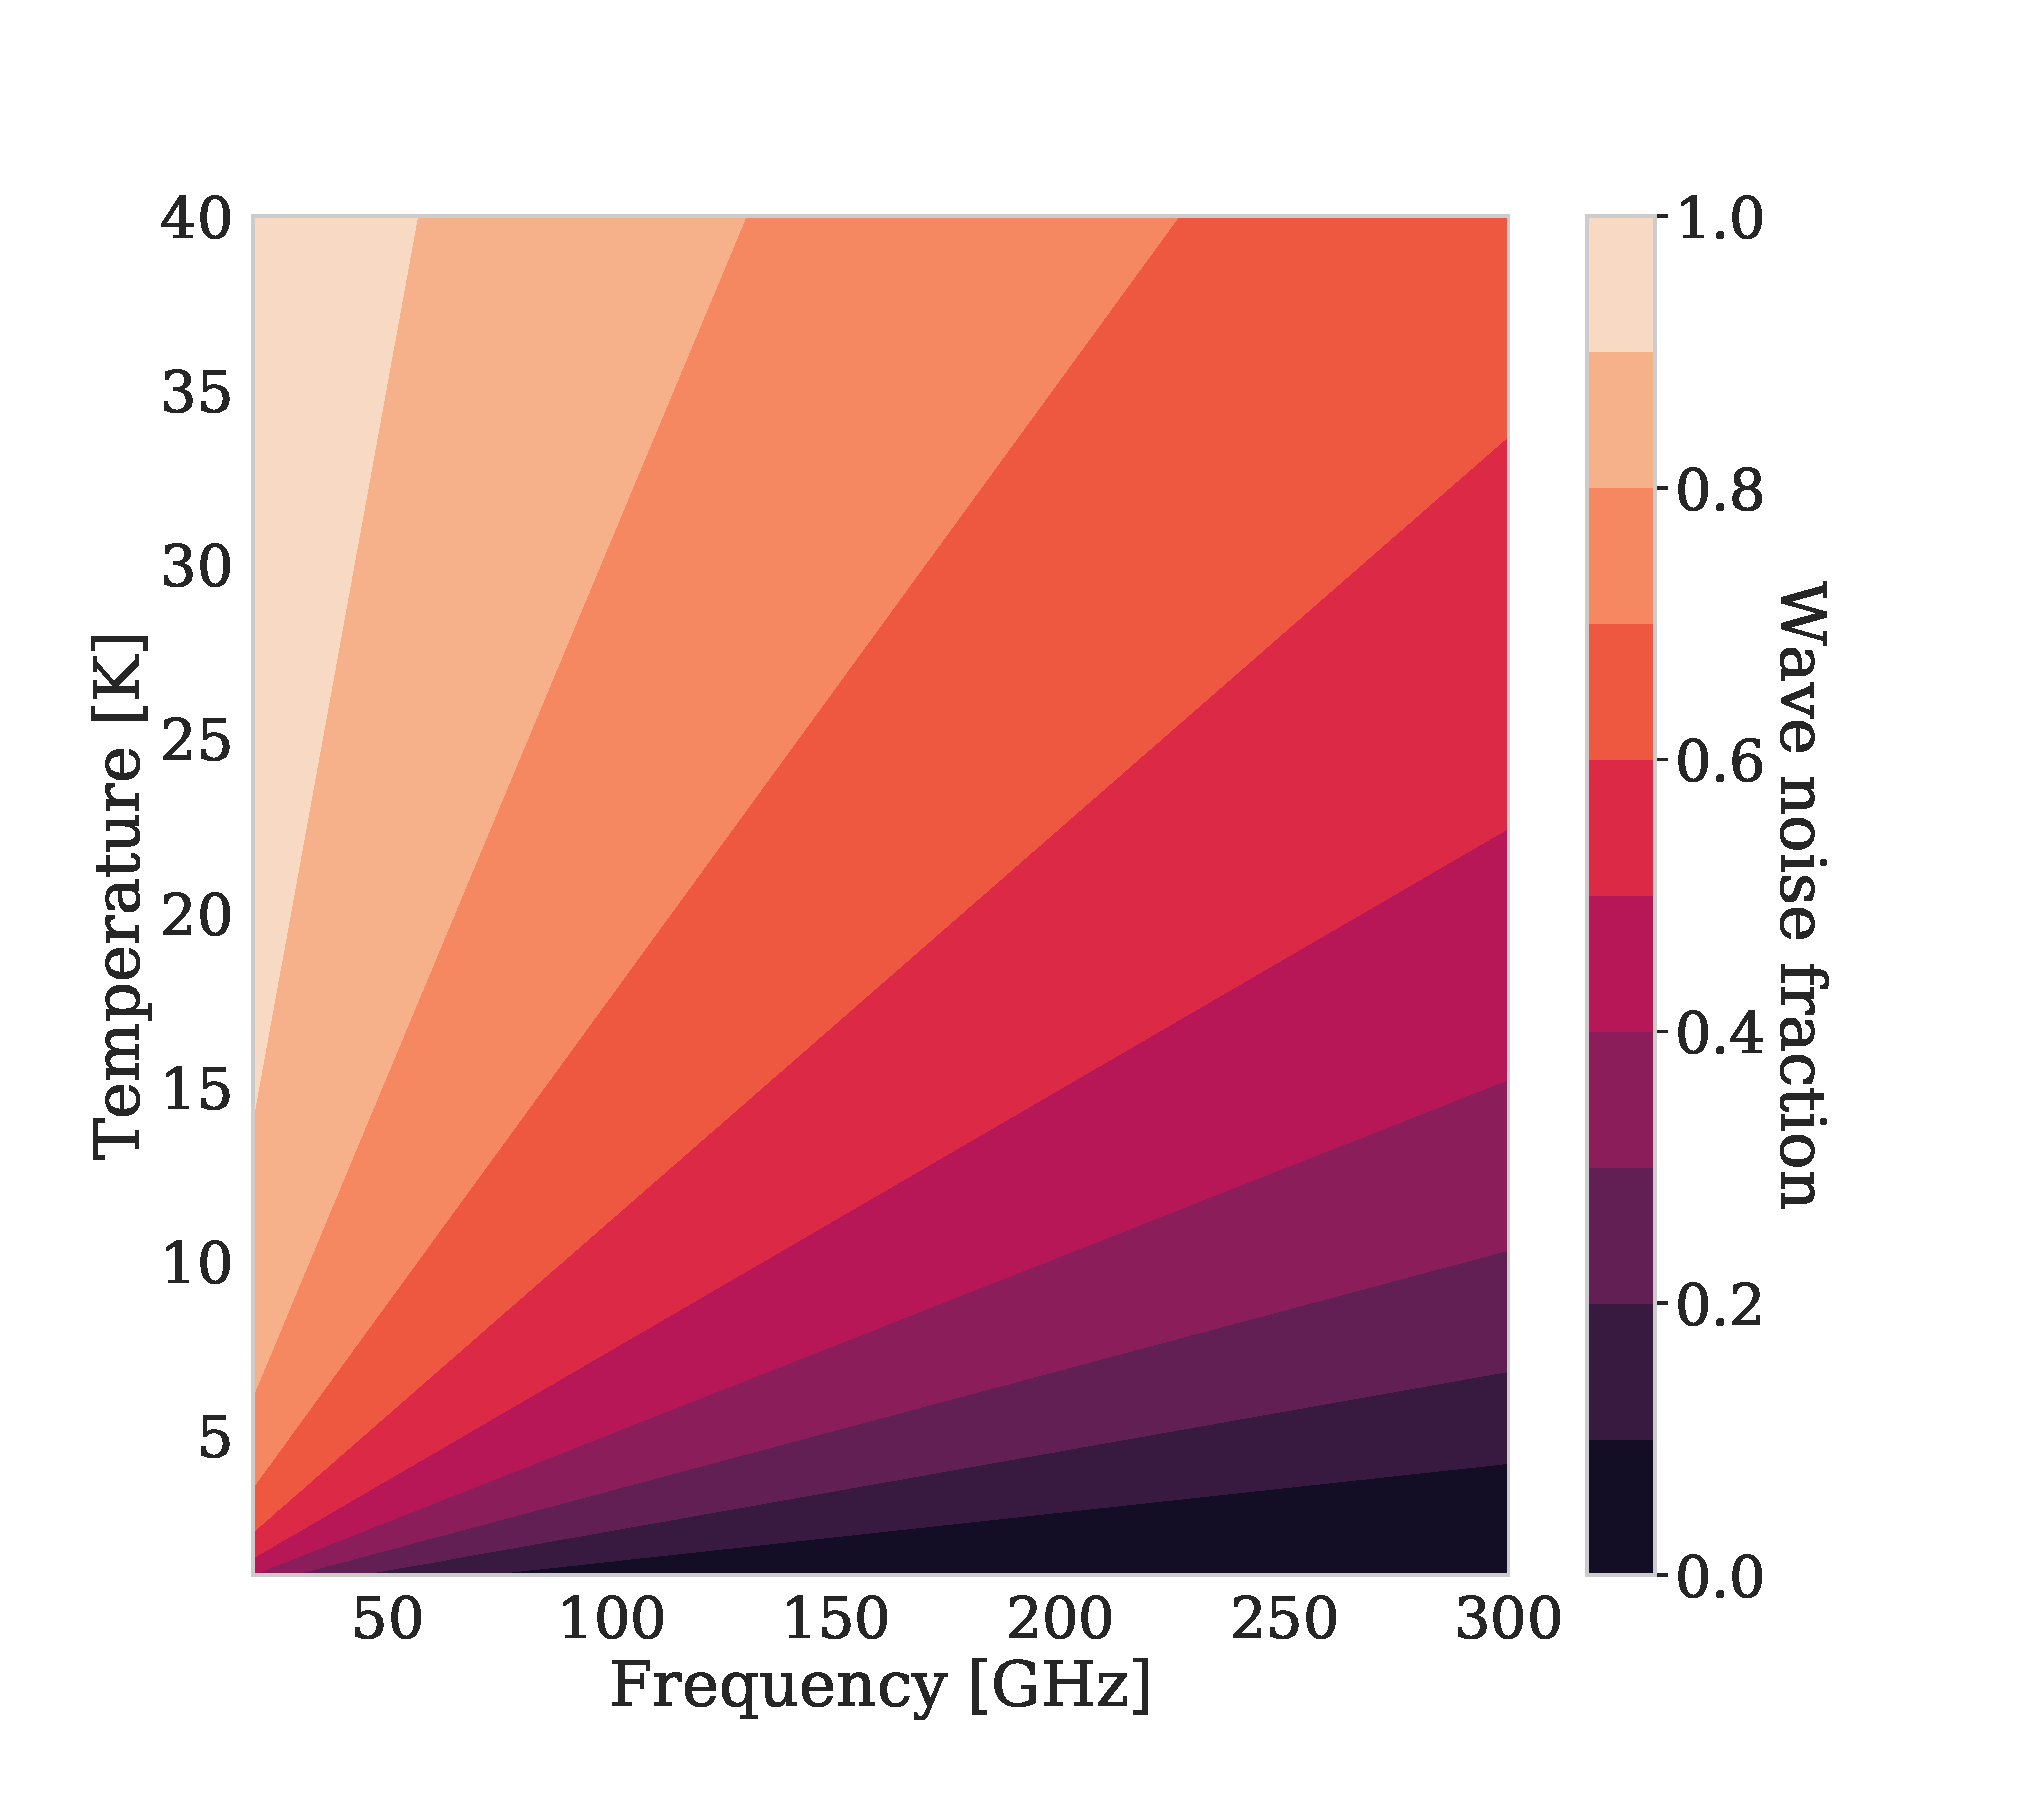
\includegraphics[width=0.65\linewidth, trim=1cm 1cm 1cm 3cm, clip]{SensitivityCalculation/Figures/bose_noise_fraction.pdf}
    \caption{Wave noise fraction, which is defined as $\mathrm{NEP_{wave}} / \sqrt{NEP_{wave}^{2} + NEP_{shot}^{2}}$, assuming a top-hat band of 20~GHz bandwidth and an optical throughput between the source and detector of 30\%.}
    \label{fig:bose_noise_fraction}
\end{figure}

The cumulative correlation coefficient $\gamma$ is given by a summation of the correlation coefficients between all $N_{\mathrm{pix}}$ detector pixels on the focal plane
\begin{equation}
    \gamma = \frac{1}{N_{\mathrm{pix}}-1} \sum_{i} \sum_{j \neq i} \gamma_{i,j}\,\, .
\end{equation}
These correlations then propagate to $\mathrm{NET_{arr}}$ by suppressing the degree to which wave noise is averaged down when inverse-variance averaging the detector data
\begin{equation}
    \mathrm{NET}_{\mathrm{arr}} = \sqrt{\frac{\mathrm{NET}^{2}_{\mathrm{shot}} + (1 + \gamma) \mathrm{NET}^{2}_{\mathrm{wave}} + 
    \mathrm{NET}^{2}_{\mathrm{g}} + \mathrm{NET}^{2}_{\mathrm{read}}}{Y N_{\mathrm{det}}}}\,\, .
\end{equation}
We can now write the array NET correlation suppression factor $\Gamma$ defined in Equation \ref{eq:net_arr} as
\begin{equation}
    \Gamma = \sqrt{1 + \frac{\gamma \, \mathrm{NET}^{2}_{\mathrm{wave}}}{\mathrm{NET}^{2}_{\mathrm{shot}} + \mathrm{NET}^{2}_{\mathrm{wave}} + \mathrm{NET}^{2}_{\mathrm{g}} + 
    \mathrm{NET}^{2}_{\mathrm{read}}}} \; .
    \label{eq:corr_fact}
\end{equation}
As evident in Equation~\ref{eq:corr_fact}, the impact of correlations on array NET depends not only on the the HBT coefficient but on the contribution of wave noise to the total noise in the system and on the optical correlation factor $\gamma$, further emphasizing the importance of an accurate $P_{\mathrm{opt}}$ estimate to an accurate estimate of $\Gamma$.

%%%%%%%%%%%%%%%%%%%%%%%%%%%%%%%%
%%%%%%%%%%%%%%%%%%%%%%%%%%%%%%%%
%%%%%%%%%%%%%%%%%%%%%%%%%%%%%%%%

\section{$N_{\mathrm{\ell}}$ and mapping speed}
\label{sec:N_ell_mapping_speed}

As presented in Section~\ref{sec:sensitivity_calculation_net}, NET has units of $\mathrm{\mu K \sqrt{s}}$ and is a measure noise in the detector time streams referenced to fluctuations in sky temperature. It is often useful to convert this time-domain noise into \important{map depth}, or noise in a sky-map domain, which defined as
\begin{equation}
    \sigma_{\mathrm{map}} = \mathrm{NET}_{\mathrm{arr}} \sqrt{\frac{4 \pi \left( 10,800 / \pi \right)^{2} f_{\mathrm{sky}}}{\eta_{\mathrm{obs}} t_{\mathrm{obs}}}} \, ,
    \label{eq:map_depth}
\end{equation}
in units of $\mathrm{K - arcmin}$. Here, we convert NET from a temporal spectral density to a spatial spectral density by dividing by the square root of \important{integration time}, which is the product of the observatory's lifetime $t_{\mathrm{obs}}$ and its observation efficiency $\eta_{\mathrm{obs}}$, and multiplying by the square root of sky area, which the total number of arcminutes on the sky multiplied the observed sky fraction $f_{\mathrm{sky}}$. In addition to having low NETs, map depth is improved by both integrating for longer and by observing smaller sky patches. However, as shown in Equation~\ref{eq:cosmic_variance}, a smaller sky fraction leads to a larger cosmic variance, and therefore the trade-off between map depth and sky coverage must be carefully considered when optimizing observation strategies to measure large angular scales. 

The figure of merit for power spectrum sensitivity is \important{$N_{\ell}$}, which measures RMS noise in $K^{2}$ in the CMB power spectrum as a function of angular multipole number $\ell$
\begin{equation}
    \Delta C_{\ell} = \sqrt{\frac{2}{\left( 2 \ell + 1 \right) f_{\mathrm{sky}}}} \left( C_{\ell} + N_{\ell} \right) \, ,
    \label{eq:N_ell_in_contex}
\end{equation}
where the first term is the cosmic variance discussed in Section~\ref{sec:cmb_power_spectrum}. $N_{\ell}$ due to white noise can in turn be written using what is often called the \important{Knox Formula}
\begin{equation}
    N_{\ell}^{\mathrm{white}} = 4 \sigma_{\mathrm{map}}^{2} e^{\ell^{2} \sigma_{\mathrm{beam}}^{2}} \, ,
    \label{eq:N_ell}
\end{equation}
where the exponential term is called the \important{beam transfer function} and $\sigma_{\mathrm{beam}}$ is the telescope's angular resolution. The degradation of noise at angular scales smaller than the beam is an important driver of the telescope's primary aperture size. For example, a large-aperture telescope with $\sigma_{\mathrm{beam}} = 0.1$~deg beam will make a much more sensitive measurement of at $\ell = 2,000$ than a small-aperture telescope with $\sigma_{\mathrm{beam}} = 1$~deg, even if the small-aperture telescope has much more sensitive detectors.

\begin{figure}[!t]
    \centering
    \subfloat[\label{fig:noise_curves:a}]{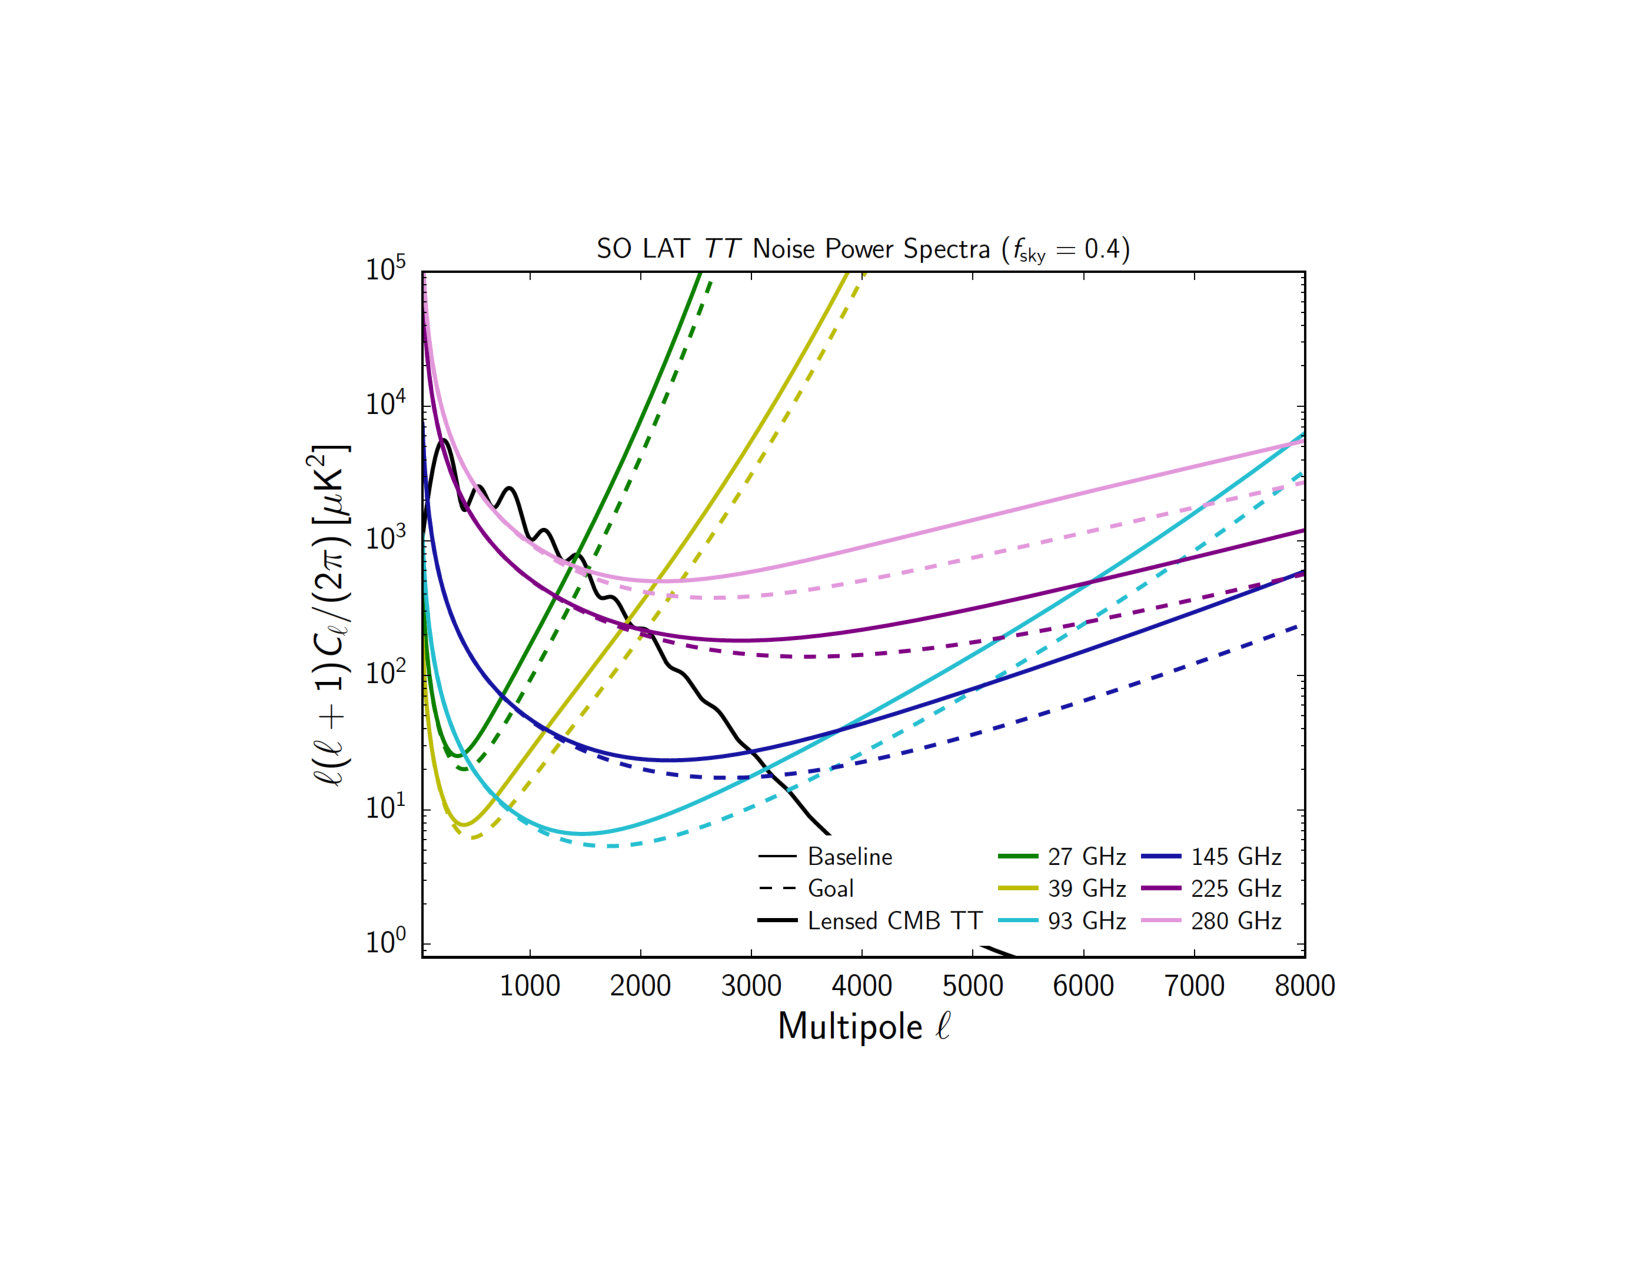
\includegraphics[width=0.48\linewidth, trim=5cm 3.8cm 4.9cm 3.8cm, clip]{SensitivityCalculation/Figures/SO_LAT_TT_noiseCurves.pdf}}
    \subfloat[\label{fig:noise_curves:b}]{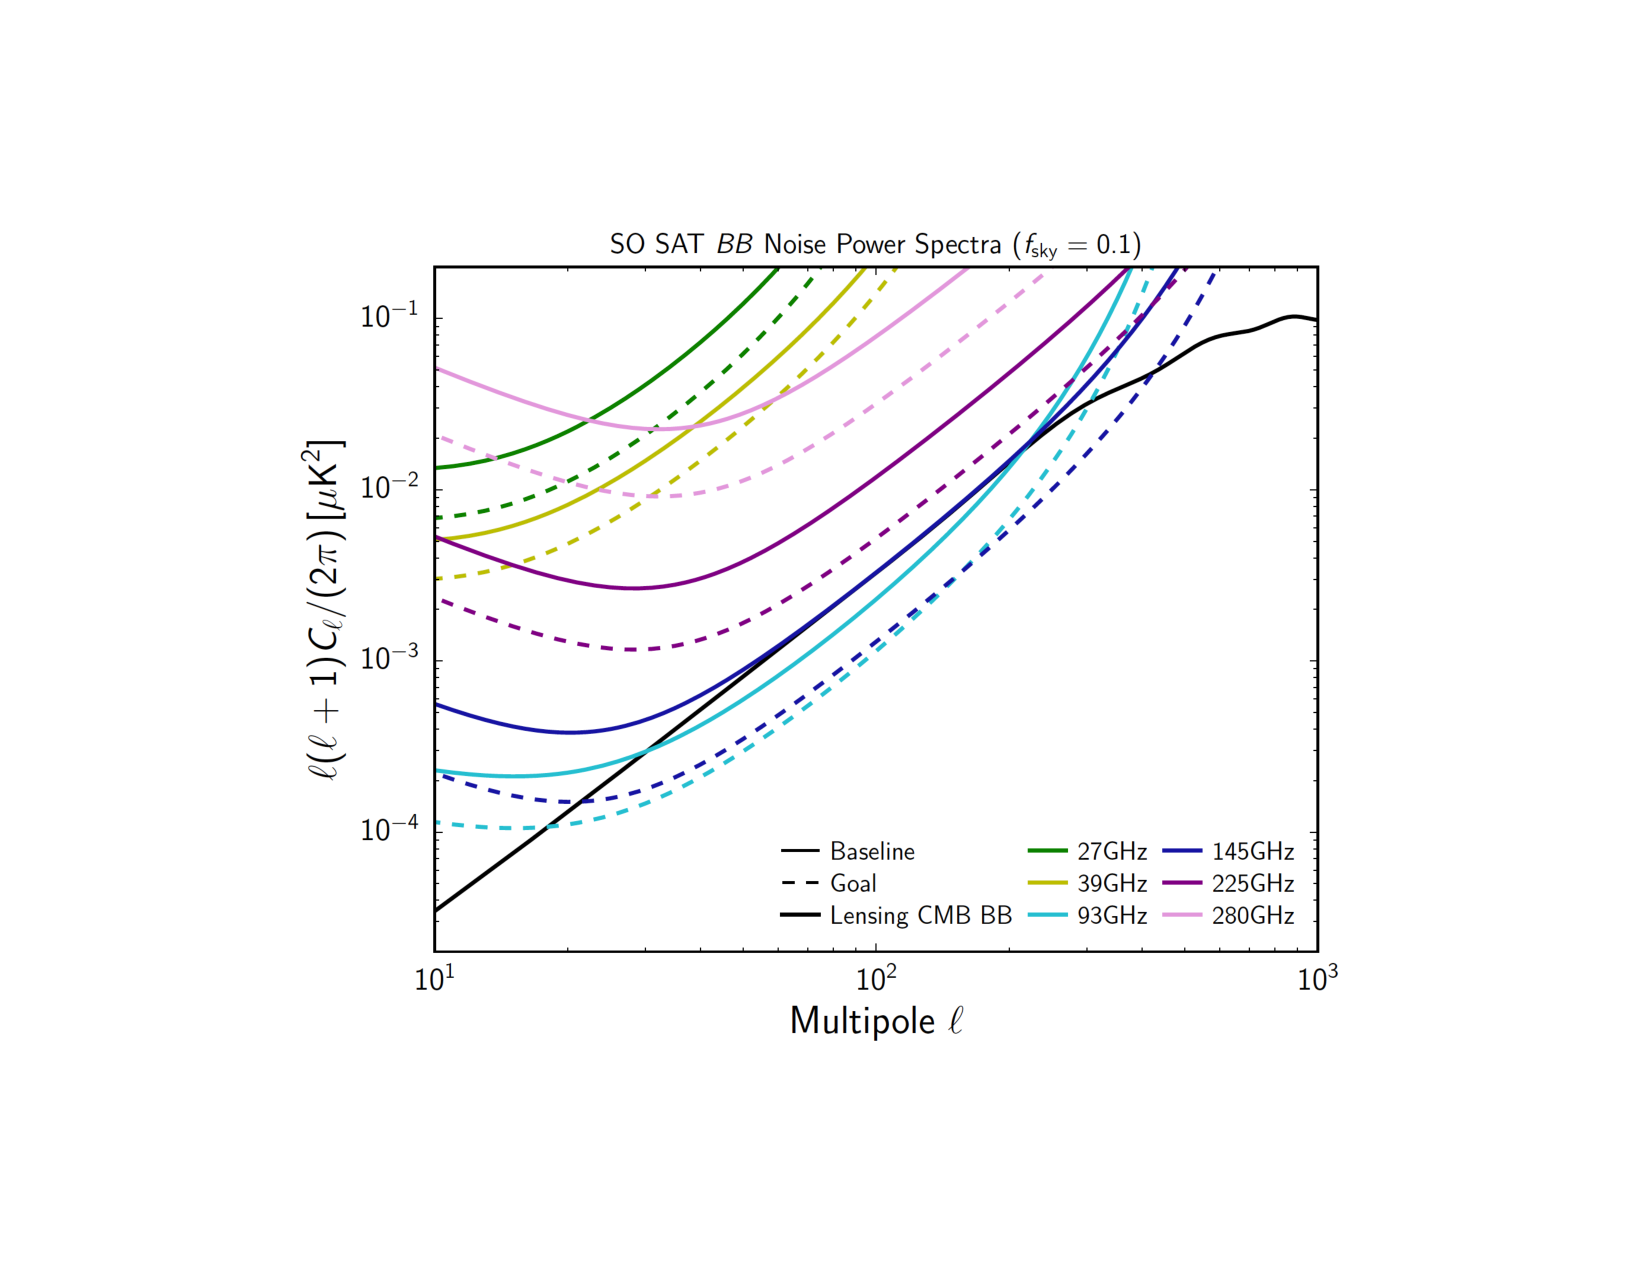
\includegraphics[width=0.48\linewidth, trim=5cm 3.8cm 4.9cm 3.8cm, clip]{SensitivityCalculation/Figures/SO_SAT_BB_noiseCurves.pdf}}
    \caption{Forecasted $N_{\ell}$ \important{noise curves} for the SO LAT in temperature and the SO SAT in polarization. The NETs used to formulate these forecasts were calculated using BoloCalc, which is presented in Chapter~\ref{ch:bolocalc}, and the $\ell$ dependencies were found using Equations~\ref{eq:N_ell} and~\ref{eq:N_ell_low_frequency_noise}.}
    \label{fig:N_ell_noise_curves}
\end{figure}

It is important to note that Equations~\ref{eq:map_depth} and ~\ref{eq:N_ell} are crude approximations, and that the conversion from NET to map depth is in general a complicated product of the instrument behavior, observation strategy, and analysis pipeline. For example, telescope scans cover the sky non-uniformly, and the ``weight'' of a given sky pixel is often proportional to its ``hit count,'' or the number of times it was observed, which is in general nontrivial. In addition, time-domain filtering in the detector time streams can lead to sensitivity in the azimuth and elevation (Earth) coordinates differing substantially, and due to a changing sky load with elevation, the depth of a patch in general depends on where in the sky it is scanned. Finally, unlike the assumptions throughout this entire chapter, noise is \textit{not} white but instead increases at low frequencies. The phenomenon is call \important{1/f noise}, and it is typically modeled in $\ell$ space as
\begin{equation}
    N_{\ell} = N_{\ell}^{\mathrm{white}} + N^{\mathrm{red}} \left( \frac{\ell}{\ell_{\mathrm{knee}}} \right)^{\alpha_{\mathrm{knee}}} \, ,
    \label{eq:N_ell_low_frequency_noise}
\end{equation}
where the $\ell$ knee $\ell_{\mathrm{knee}}$, 1/f spectral index
$\alpha_{\mathrm{knee}}$ and 1/f noise amplitude $N^{\mathrm{red}}$ are usually determined empirically.

Noting that the figure of merit for any CMB power spectrum measurement is the noise in power spectrum space, it is quite useful for CMB instrumentalists to quantify instrument sensitivity in terms of \important{mapping speed}
\begin{equation}
    \mathrm{MS} \equiv \frac{1}{\mathrm{NET_{arr}}^{2}} = \frac{N_{\mathrm{det}} Y}{\mathrm{NET_{det}}^{2}} \, .
\end{equation}
Mapping speed quantifies the number of detector-hours needed to reach a specified CMB map depth and is therefore proportional to detector yield observation efficiency. As a result, mapping speed (or mapping speed per cost) is often used as figure of merit during experiment design and optimization.

%%%%%%%%%%%%%%%%%%%%%%%%%%%%%%%%
%%%%%%%%%%%%%%%%%%%%%%%%%%%%%%%%
%%%%%%%%%%%%%%%%%%%%%%%%%%%%%%%%

\section{Discussion}
\label{sec:sensitivity_discussion}